% Relatório técnico da DSM4 (entrega final) — Sistema Multiagente de Controladoria da SMA.
% Compilar: make pdf-dsm4 (converte as figuras SVG do experimento e roda latexmk com bibtex).
% Todo número vem de numeros.tex (\V{chave} e \Tab...), gerado por tools/relatorio_numeros.py.
% Os parágrafos dos lotes de conectores e de acesso avançado (marcados "% Integrado da branch dsm4/v1.0.0") foram
% escritos a partir de docs/dsm4/ADR-011, ADR-012 e acesso-avancado.md daquela branch; os números deles saem de
% tools/relatorio_numeros.py rodado sobre o código integrado.
\documentclass[10pt,a4paper]{article}

\newcommand{\autorA}{Danrley Moreira Ribeiro}
\newcommand{\matA}{23102664}
\newcommand{\autorB}{Jiliard Mai Peifer}
\newcommand{\matB}{23103129}
\newcommand{\repoURL}{https://github.com/danrley-ribeiro/fin-dept-multiagents-project}
\newcommand{\docsURL}{https://fin-dept-multiagents-project.readthedocs.io}

\usepackage[T1]{fontenc}
\usepackage[utf8]{inputenc}
\usepackage[brazil]{babel}
\usepackage[default,semibold]{sourcesanspro}
\usepackage[a4paper, left=1.6cm, right=1.6cm, top=1.8cm, bottom=1.8cm, headsep=0.5cm, footskip=0.8cm]{geometry}
\usepackage{xcolor}
\usepackage{amsmath, amssymb}
\usepackage{microtype}
\usepackage{array, booktabs, tabularx, makecell}
\usepackage{enumitem}
\usepackage{titlesec}
\usepackage{fancyhdr}
\usepackage{ragged2e}
\usepackage{graphicx}
\usepackage{caption}
\usepackage{float}
\usepackage{tikz}
\usetikzlibrary{arrows.meta, positioning, calc, fit, backgrounds}
\usepackage{csquotes}
\usepackage[backend=bibtex, style=authoryear, maxcitenames=2, uniquename=false, uniquelist=false, dashed=false]{biblatex}
\addbibresource{referencias.bib}
\usepackage{newunicodechar}
\newunicodechar{→}{\ensuremath{\rightarrow}}
\newunicodechar{×}{\ensuremath{\times}}
\newunicodechar{≥}{\ensuremath{\geq}}
\newunicodechar{≤}{\ensuremath{\leq}}
\usepackage[hidelinks, pdfusetitle]{hyperref}
\hypersetup{pdftitle={DSM4 — Sistema Multiagente de Controladoria: relatório técnico},
            pdfauthor={\autorA, \autorB}, pdfsubject={INE5628 — Entrega final}}

% commit a407a31, 13/11/2026
% Gerado por tools/relatorio_numeros.py; não edite à mão.
\providecommand{\V}[1]{\ifcsname V@#1\endcsname\csname V@#1\endcsname\else\textbf{??\detokenize{#1}??}\PackageWarning{numeros}{chave indefinida: #1}\fi}
\expandafter\newcommand\csname V@abl.sem_cognicao_local.com\endcsname{50,0\%}
\expandafter\newcommand\csname V@abl.sem_cognicao_local.dif\endcsname{$-$10,0 pp}
\expandafter\newcommand\csname V@abl.sem_cognicao_local.p\endcsname{0,250}
\expandafter\newcommand\csname V@abl.sem_cognicao_local.seeds\endcsname{3}
\expandafter\newcommand\csname V@abl.sem_cognicao_local.sem\endcsname{40,0\%}
\expandafter\newcommand\csname V@abl.sem_correcao.com\endcsname{2,00}
\expandafter\newcommand\csname V@abl.sem_correcao.dif\endcsname{$-$2,00}
\expandafter\newcommand\csname V@abl.sem_correcao.p\endcsname{$<$\,0,001}
\expandafter\newcommand\csname V@abl.sem_correcao.publicacao\endcsname{66,7\%}
\expandafter\newcommand\csname V@abl.sem_correcao.seeds\endcsname{30}
\expandafter\newcommand\csname V@abl.sem_correcao.sem\endcsname{0,00}
\expandafter\newcommand\csname V@abl.sem_negociacao.com\endcsname{50,0\%}
\expandafter\newcommand\csname V@abl.sem_negociacao.dif\endcsname{0,0 pp}
\expandafter\newcommand\csname V@abl.sem_negociacao.p\endcsname{---}
\expandafter\newcommand\csname V@abl.sem_negociacao.seeds\endcsname{0}
\expandafter\newcommand\csname V@abl.sem_negociacao.sem\endcsname{50,0\%}
\expandafter\newcommand\csname V@abl.sem_reenvio.com\endcsname{61,7\%}
\expandafter\newcommand\csname V@abl.sem_reenvio.dif\endcsname{$-$30,0 pp}
\expandafter\newcommand\csname V@abl.sem_reenvio.p\endcsname{$<$\,0,001}
\expandafter\newcommand\csname V@abl.sem_reenvio.seeds\endcsname{13}
\expandafter\newcommand\csname V@abl.sem_reenvio.sem\endcsname{31,7\%}
\expandafter\newcommand\csname V@abl.sem_reserva.com\endcsname{1,00}
\expandafter\newcommand\csname V@abl.sem_reserva.dif\endcsname{1,00}
\expandafter\newcommand\csname V@abl.sem_reserva.p\endcsname{$<$\,0,001}
\expandafter\newcommand\csname V@abl.sem_reserva.seeds\endcsname{30}
\expandafter\newcommand\csname V@abl.sem_reserva.sem\endcsname{2,00}
\expandafter\newcommand\csname V@ataques.acesso\endcsname{15}
\expandafter\newcommand\csname V@ataques.acesso.rejeitados\endcsname{15}
\expandafter\newcommand\csname V@ataques.acesso_avancado\endcsname{---}
\expandafter\newcommand\csname V@ataques.acesso_avancado.rejeitados\endcsname{---}
\expandafter\newcommand\csname V@ataques.barramento\endcsname{14}
\expandafter\newcommand\csname V@ataques.barramento.rejeitados\endcsname{14}
\expandafter\newcommand\csname V@cenarios.basico\endcsname{28}
\expandafter\newcommand\csname V@cenarios.dsm3\endcsname{37}
\expandafter\newcommand\csname V@cenarios.dsm4\endcsname{16}
\expandafter\newcommand\csname V@cenarios.llm\endcsname{7}
\expandafter\newcommand\csname V@cenarios.local\endcsname{18}
\expandafter\newcommand\csname V@cenarios.total\endcsname{53}
\expandafter\newcommand\csname V@cenarios.verificados\endcsname{53}
\expandafter\newcommand\csname V@coletivo.sma_basico.decisoes\endcsname{17,2}
\expandafter\newcommand\csname V@coletivo.sma_basico.distribuicao\endcsname{77\%}
\expandafter\newcommand\csname V@coletivo.sma_local.decisoes\endcsname{24,7}
\expandafter\newcommand\csname V@coletivo.sma_local.distribuicao\endcsname{84\%}
\expandafter\newcommand\csname V@coletivo.wf_equivalente.decisoes\endcsname{6,1}
\expandafter\newcommand\csname V@coletivo.wf_equivalente.distribuicao\endcsname{0\%}
\expandafter\newcommand\csname V@exp.alfa\endcsname{0,05}
\expandafter\newcommand\csname V@exp.ataques.aceitos\endcsname{9}
\expandafter\newcommand\csname V@exp.ataques.indevidos\endcsname{0}
\expandafter\newcommand\csname V@exp.ataques.sem_premissa\endcsname{9}
\expandafter\newcommand\csname V@exp.ataques.tentados\endcsname{2.227}
\expandafter\newcommand\csname V@exp.bloco.A\endcsname{6.000}
\expandafter\newcommand\csname V@exp.bloco.B\endcsname{2.160}
\expandafter\newcommand\csname V@exp.bloco.C\endcsname{1.080}
\expandafter\newcommand\csname V@exp.bloco.D\endcsname{120}
\expandafter\newcommand\csname V@exp.condicoes\endcsname{9}
\expandafter\newcommand\csname V@exp.erros\endcsname{0}
\expandafter\newcommand\csname V@exp.execucoes\endcsname{9.360}
\expandafter\newcommand\csname V@exp.familias\endcsname{9}
\expandafter\newcommand\csname V@exp.p_plantio\endcsname{0,35}
\expandafter\newcommand\csname V@exp.plantios\endcsname{7}
\expandafter\newcommand\csname V@exp.portes\endcsname{4}
\expandafter\newcommand\csname V@exp.reamostragens\endcsname{2.000}
\expandafter\newcommand\csname V@exp.seed.max\endcsname{30}
\expandafter\newcommand\csname V@exp.seed.min\endcsname{1}
\expandafter\newcommand\csname V@exp.seeds\endcsname{30}
\expandafter\newcommand\csname V@exp.sem_resposta\endcsname{0}
\expandafter\newcommand\csname V@exp.sha\endcsname{952af6eb}
\expandafter\newcommand\csname V@exp.sha.completo\endcsname{952af6ebbbd76974e655af7083503e1a9e73af2d5daa0c4a71a7fc929d5cfc12}
\expandafter\newcommand\csname V@exp.sma.execucoes\endcsname{6.480}
\expandafter\newcommand\csname V@exp.testes\endcsname{60}
\expandafter\newcommand\csname V@exp.violacoes\endcsname{0}
\expandafter\newcommand\csname V@gerado.commit\endcsname{a407a31}
\expandafter\newcommand\csname V@gerado.data\endcsname{13/11/2026}
\expandafter\newcommand\csname V@invariantes\endcsname{8}
\expandafter\newcommand\csname V@modelos.agents\endcsname{6}
\expandafter\newcommand\csname V@modelos.components\endcsname{46}
\expandafter\newcommand\csname V@modelos.metrics\endcsname{27}
\expandafter\newcommand\csname V@modelos.norms\endcsname{15}
\expandafter\newcommand\csname V@modelos.protocols\endcsname{6}
\expandafter\newcommand\csname V@modelos.roles\endcsname{11}
\expandafter\newcommand\csname V@modelos.services\endcsname{9}
\expandafter\newcommand\csname V@r1.abl.reenvio.com\endcsname{40,0\%}
\expandafter\newcommand\csname V@r1.abl.reenvio.sem\endcsname{28,3\%}
\expandafter\newcommand\csname V@r1.ataques\endcsname{1.735}
\expandafter\newcommand\csname V@r1.commit\endcsname{cfa6b6f}
\expandafter\newcommand\csname V@r1.inv03\endcsname{165}
\expandafter\newcommand\csname V@r1.lat.combinadas\endcsname{43,7}
\expandafter\newcommand\csname V@r1.lat.combinadas.n\endcsname{28}
\expandafter\newcommand\csname V@r1.rq2.combinadas\endcsname{45,4\%}
\expandafter\newcommand\csname V@r1.rq2.combinadas.resposta\endcsname{83,3\%}
\expandafter\newcommand\csname V@r1.rq2.humano_lento\endcsname{75,8\%}
\expandafter\newcommand\csname V@r1.rq2.humano_lento.resposta\endcsname{100\%}
\expandafter\newcommand\csname V@r1.rq2.indisponibilidade\endcsname{92,1\%}
\expandafter\newcommand\csname V@r1.rq2.indisponibilidade.resposta\endcsname{95,0\%}
\expandafter\newcommand\csname V@r1.rq2.perda_alta\endcsname{22,5\%}
\expandafter\newcommand\csname V@r1.rq2.perda_alta.resposta\endcsname{52,9\%}
\expandafter\newcommand\csname V@r1.rq2.perda_baixa\endcsname{80,0\%}
\expandafter\newcommand\csname V@r1.rq2.perda_baixa.resposta\endcsname{88,8\%}
\expandafter\newcommand\csname V@r1.rq2.perda_media\endcsname{48,8\%}
\expandafter\newcommand\csname V@r1.rq2.perda_media.resposta\endcsname{73,8\%}
\expandafter\newcommand\csname V@r1.rq4.combinadas.mesmo.pct\endcsname{26\%}
\expandafter\newcommand\csname V@r1.rq4.combinadas.sem_resposta\endcsname{40}
\expandafter\newcommand\csname V@r1.rq4.indisponibilidade.mesmo.pct\endcsname{67\%}
\expandafter\newcommand\csname V@r1.rq4.indisponibilidade.sem_resposta\endcsname{12}
\expandafter\newcommand\csname V@r1.rq4.perda_alta.mesmo.pct\endcsname{15\%}
\expandafter\newcommand\csname V@r1.rq4.perda_alta.sem_resposta\endcsname{113}
\expandafter\newcommand\csname V@r1.rq4.perda_baixa.mesmo.pct\endcsname{54\%}
\expandafter\newcommand\csname V@r1.rq4.perda_baixa.sem_resposta\endcsname{27}
\expandafter\newcommand\csname V@r1.rq4.perda_media.mesmo.pct\endcsname{35\%}
\expandafter\newcommand\csname V@r1.rq4.perda_media.sem_resposta\endcsname{63}
\expandafter\newcommand\csname V@r1.rq6.atacadas\endcsname{97}
\expandafter\newcommand\csname V@r1.sha\endcsname{c5a4e032}
\expandafter\newcommand\csname V@r1.violacoes\endcsname{807}
\expandafter\newcommand\csname V@r2.commit\endcsname{ab4cc3a}
\expandafter\newcommand\csname V@rq1.min.cliff\endcsname{0,33}
\expandafter\newcommand\csname V@rq1.min.criticas.cliff\endcsname{$-$0,93}
\expandafter\newcommand\csname V@rq1.min.dif\endcsname{+38,3 pp}
\expandafter\newcommand\csname V@rq1.min.dif.ic\endcsname{[23,3; 53,3]}
\expandafter\newcommand\csname V@rq1.min.p\endcsname{$<$\,0,001}
\expandafter\newcommand\csname V@rq1.pares\endcsname{240}
\expandafter\newcommand\csname V@rq1.pares.diferentes\endcsname{0}
\expandafter\newcommand\csname V@rq1.sma_basico.classificacao_correta\endcsname{75,0\%}
\expandafter\newcommand\csname V@rq1.sma_basico.classificacao_correta.ic\endcsname{[63,3\%; 85,8\%]}
\expandafter\newcommand\csname V@rq1.sma_basico.concluida\endcsname{100\%}
\expandafter\newcommand\csname V@rq1.sma_basico.concluida.ic\endcsname{[100\%; 100\%]}
\expandafter\newcommand\csname V@rq1.sma_basico.conformidade_correta\endcsname{100\%}
\expandafter\newcommand\csname V@rq1.sma_basico.conformidade_correta.ic\endcsname{[100\%; 100\%]}
\expandafter\newcommand\csname V@rq1.sma_basico.criticas\endcsname{0,00}
\expandafter\newcommand\csname V@rq1.sma_basico.criticas.ic\endcsname{[0,00; 0,00]}
\expandafter\newcommand\csname V@rq1.sma_basico.dre_correta\endcsname{100\%}
\expandafter\newcommand\csname V@rq1.sma_basico.dre_correta.ic\endcsname{[100\%; 100\%]}
\expandafter\newcommand\csname V@rq1.sma_basico.sinalizacao_correta\endcsname{89,2\%}
\expandafter\newcommand\csname V@rq1.sma_basico.sinalizacao_correta.ic\endcsname{[85,0\%; 93,3\%]}
\expandafter\newcommand\csname V@rq1.sma_local.classificacao_correta\endcsname{75,0\%}
\expandafter\newcommand\csname V@rq1.sma_local.classificacao_correta.ic\endcsname{[63,3\%; 85,8\%]}
\expandafter\newcommand\csname V@rq1.sma_local.concluida\endcsname{100\%}
\expandafter\newcommand\csname V@rq1.sma_local.concluida.ic\endcsname{[100\%; 100\%]}
\expandafter\newcommand\csname V@rq1.sma_local.conformidade_correta\endcsname{100\%}
\expandafter\newcommand\csname V@rq1.sma_local.conformidade_correta.ic\endcsname{[100\%; 100\%]}
\expandafter\newcommand\csname V@rq1.sma_local.criticas\endcsname{0,00}
\expandafter\newcommand\csname V@rq1.sma_local.criticas.ic\endcsname{[0,00; 0,00]}
\expandafter\newcommand\csname V@rq1.sma_local.dre_correta\endcsname{100\%}
\expandafter\newcommand\csname V@rq1.sma_local.dre_correta.ic\endcsname{[100\%; 100\%]}
\expandafter\newcommand\csname V@rq1.sma_local.sinalizacao_correta\endcsname{89,2\%}
\expandafter\newcommand\csname V@rq1.sma_local.sinalizacao_correta.ic\endcsname{[85,0\%; 93,3\%]}
\expandafter\newcommand\csname V@rq1.wf_equivalente.classificacao_correta\endcsname{75,0\%}
\expandafter\newcommand\csname V@rq1.wf_equivalente.classificacao_correta.ic\endcsname{[63,3\%; 85,8\%]}
\expandafter\newcommand\csname V@rq1.wf_equivalente.concluida\endcsname{100\%}
\expandafter\newcommand\csname V@rq1.wf_equivalente.concluida.ic\endcsname{[100\%; 100\%]}
\expandafter\newcommand\csname V@rq1.wf_equivalente.conformidade_correta\endcsname{100\%}
\expandafter\newcommand\csname V@rq1.wf_equivalente.conformidade_correta.ic\endcsname{[100\%; 100\%]}
\expandafter\newcommand\csname V@rq1.wf_equivalente.criticas\endcsname{0,00}
\expandafter\newcommand\csname V@rq1.wf_equivalente.criticas.ic\endcsname{[0,00; 0,00]}
\expandafter\newcommand\csname V@rq1.wf_equivalente.dre_correta\endcsname{100\%}
\expandafter\newcommand\csname V@rq1.wf_equivalente.dre_correta.ic\endcsname{[100\%; 100\%]}
\expandafter\newcommand\csname V@rq1.wf_equivalente.sinalizacao_correta\endcsname{89,2\%}
\expandafter\newcommand\csname V@rq1.wf_equivalente.sinalizacao_correta.ic\endcsname{[85,0\%; 93,3\%]}
\expandafter\newcommand\csname V@rq1.wf_minimo.classificacao_correta\endcsname{36,7\%}
\expandafter\newcommand\csname V@rq1.wf_minimo.classificacao_correta.ic\endcsname{[20,0\%; 53,3\%]}
\expandafter\newcommand\csname V@rq1.wf_minimo.concluida\endcsname{100\%}
\expandafter\newcommand\csname V@rq1.wf_minimo.concluida.ic\endcsname{[100\%; 100\%]}
\expandafter\newcommand\csname V@rq1.wf_minimo.conformidade_correta\endcsname{100\%}
\expandafter\newcommand\csname V@rq1.wf_minimo.conformidade_correta.ic\endcsname{[100\%; 100\%]}
\expandafter\newcommand\csname V@rq1.wf_minimo.criticas\endcsname{0,68}
\expandafter\newcommand\csname V@rq1.wf_minimo.criticas.ic\endcsname{[0,55; 0,83]}
\expandafter\newcommand\csname V@rq1.wf_minimo.dre_correta\endcsname{100\%}
\expandafter\newcommand\csname V@rq1.wf_minimo.dre_correta.ic\endcsname{[100\%; 100\%]}
\expandafter\newcommand\csname V@rq1.wf_minimo.sinalizacao_correta\endcsname{51,7\%}
\expandafter\newcommand\csname V@rq1.wf_minimo.sinalizacao_correta.ic\endcsname{[35,0\%; 68,3\%]}
\expandafter\newcommand\csname V@rq2.combinadas.cliff\endcsname{$-$0,45}
\expandafter\newcommand\csname V@rq2.combinadas.dif\endcsname{$-$25,0 pp}
\expandafter\newcommand\csname V@rq2.combinadas.dif.ic\endcsname{[$-$37,1; $-$14,2]}
\expandafter\newcommand\csname V@rq2.combinadas.p\endcsname{$<$\,0,001}
\expandafter\newcommand\csname V@rq2.combinadas.seeds\endcsname{14}
\expandafter\newcommand\csname V@rq2.combinadas.sma_basico\endcsname{50,8\%}
\expandafter\newcommand\csname V@rq2.combinadas.sma_basico.criticas\endcsname{0}
\expandafter\newcommand\csname V@rq2.combinadas.sma_basico.ic\endcsname{[40,0\%; 61,7\%]}
\expandafter\newcommand\csname V@rq2.combinadas.sma_basico.resposta\endcsname{100\%}
\expandafter\newcommand\csname V@rq2.combinadas.sma_local\endcsname{57,9\%}
\expandafter\newcommand\csname V@rq2.combinadas.sma_local.criticas\endcsname{0}
\expandafter\newcommand\csname V@rq2.combinadas.sma_local.ic\endcsname{[45,8\%; 70,0\%]}
\expandafter\newcommand\csname V@rq2.combinadas.sma_local.resposta\endcsname{100\%}
\expandafter\newcommand\csname V@rq2.combinadas.wf_equivalente\endcsname{75,8\%}
\expandafter\newcommand\csname V@rq2.combinadas.wf_equivalente.criticas\endcsname{0}
\expandafter\newcommand\csname V@rq2.combinadas.wf_equivalente.ic\endcsname{[67,1\%; 84,2\%]}
\expandafter\newcommand\csname V@rq2.combinadas.wf_equivalente.resposta\endcsname{100\%}
\expandafter\newcommand\csname V@rq2.combinadas_ataque.cliff\endcsname{$-$0,45}
\expandafter\newcommand\csname V@rq2.combinadas_ataque.dif\endcsname{$-$25,0 pp}
\expandafter\newcommand\csname V@rq2.combinadas_ataque.dif.ic\endcsname{[$-$37,1; $-$14,2]}
\expandafter\newcommand\csname V@rq2.combinadas_ataque.p\endcsname{$<$\,0,001}
\expandafter\newcommand\csname V@rq2.combinadas_ataque.seeds\endcsname{14}
\expandafter\newcommand\csname V@rq2.combinadas_ataque.sma_basico\endcsname{50,8\%}
\expandafter\newcommand\csname V@rq2.combinadas_ataque.sma_basico.criticas\endcsname{0}
\expandafter\newcommand\csname V@rq2.combinadas_ataque.sma_basico.ic\endcsname{[40,0\%; 61,7\%]}
\expandafter\newcommand\csname V@rq2.combinadas_ataque.sma_basico.resposta\endcsname{100\%}
\expandafter\newcommand\csname V@rq2.combinadas_ataque.sma_local\endcsname{57,9\%}
\expandafter\newcommand\csname V@rq2.combinadas_ataque.sma_local.criticas\endcsname{0}
\expandafter\newcommand\csname V@rq2.combinadas_ataque.sma_local.ic\endcsname{[45,8\%; 70,0\%]}
\expandafter\newcommand\csname V@rq2.combinadas_ataque.sma_local.resposta\endcsname{100\%}
\expandafter\newcommand\csname V@rq2.combinadas_ataque.wf_equivalente\endcsname{75,8\%}
\expandafter\newcommand\csname V@rq2.combinadas_ataque.wf_equivalente.criticas\endcsname{0}
\expandafter\newcommand\csname V@rq2.combinadas_ataque.wf_equivalente.ic\endcsname{[67,1\%; 84,2\%]}
\expandafter\newcommand\csname V@rq2.combinadas_ataque.wf_equivalente.resposta\endcsname{100\%}
\expandafter\newcommand\csname V@rq2.humano_lento.cliff\endcsname{0,00}
\expandafter\newcommand\csname V@rq2.humano_lento.dif\endcsname{0,0 pp}
\expandafter\newcommand\csname V@rq2.humano_lento.dif.ic\endcsname{[0,0; 0,0]}
\expandafter\newcommand\csname V@rq2.humano_lento.p\endcsname{---}
\expandafter\newcommand\csname V@rq2.humano_lento.seeds\endcsname{0}
\expandafter\newcommand\csname V@rq2.humano_lento.sma_basico\endcsname{75,8\%}
\expandafter\newcommand\csname V@rq2.humano_lento.sma_basico.criticas\endcsname{0}
\expandafter\newcommand\csname V@rq2.humano_lento.sma_basico.ic\endcsname{[67,1\%; 84,2\%]}
\expandafter\newcommand\csname V@rq2.humano_lento.sma_basico.resposta\endcsname{100\%}
\expandafter\newcommand\csname V@rq2.humano_lento.sma_local\endcsname{75,8\%}
\expandafter\newcommand\csname V@rq2.humano_lento.sma_local.criticas\endcsname{0}
\expandafter\newcommand\csname V@rq2.humano_lento.sma_local.ic\endcsname{[67,1\%; 84,2\%]}
\expandafter\newcommand\csname V@rq2.humano_lento.sma_local.resposta\endcsname{100\%}
\expandafter\newcommand\csname V@rq2.humano_lento.wf_equivalente\endcsname{75,8\%}
\expandafter\newcommand\csname V@rq2.humano_lento.wf_equivalente.criticas\endcsname{0}
\expandafter\newcommand\csname V@rq2.humano_lento.wf_equivalente.ic\endcsname{[67,1\%; 84,2\%]}
\expandafter\newcommand\csname V@rq2.humano_lento.wf_equivalente.resposta\endcsname{100\%}
\expandafter\newcommand\csname V@rq2.indisponibilidade.cliff\endcsname{$-$0,07}
\expandafter\newcommand\csname V@rq2.indisponibilidade.dif\endcsname{$-$2,9 pp}
\expandafter\newcommand\csname V@rq2.indisponibilidade.dif.ic\endcsname{[$-$7,9; 0,0]}
\expandafter\newcommand\csname V@rq2.indisponibilidade.p\endcsname{0,500}
\expandafter\newcommand\csname V@rq2.indisponibilidade.seeds\endcsname{2}
\expandafter\newcommand\csname V@rq2.indisponibilidade.sma_basico\endcsname{97,1\%}
\expandafter\newcommand\csname V@rq2.indisponibilidade.sma_basico.criticas\endcsname{0}
\expandafter\newcommand\csname V@rq2.indisponibilidade.sma_basico.ic\endcsname{[92,1\%; 100\%]}
\expandafter\newcommand\csname V@rq2.indisponibilidade.sma_basico.resposta\endcsname{100\%}
\expandafter\newcommand\csname V@rq2.indisponibilidade.sma_local\endcsname{98,3\%}
\expandafter\newcommand\csname V@rq2.indisponibilidade.sma_local.criticas\endcsname{0}
\expandafter\newcommand\csname V@rq2.indisponibilidade.sma_local.ic\endcsname{[95,8\%; 100\%]}
\expandafter\newcommand\csname V@rq2.indisponibilidade.sma_local.resposta\endcsname{100\%}
\expandafter\newcommand\csname V@rq2.indisponibilidade.wf_equivalente\endcsname{100\%}
\expandafter\newcommand\csname V@rq2.indisponibilidade.wf_equivalente.criticas\endcsname{0}
\expandafter\newcommand\csname V@rq2.indisponibilidade.wf_equivalente.ic\endcsname{[100\%; 100\%]}
\expandafter\newcommand\csname V@rq2.indisponibilidade.wf_equivalente.resposta\endcsname{100\%}
\expandafter\newcommand\csname V@rq2.ordem.baixa_media.p\endcsname{$<$\,0,001}
\expandafter\newcommand\csname V@rq2.ordem.media_alta.p\endcsname{$<$\,0,001}
\expandafter\newcommand\csname V@rq2.perda_alta.cliff\endcsname{$-$0,93}
\expandafter\newcommand\csname V@rq2.perda_alta.dif\endcsname{$-$67,5 pp}
\expandafter\newcommand\csname V@rq2.perda_alta.dif.ic\endcsname{[$-$78,8; $-$55,8]}
\expandafter\newcommand\csname V@rq2.perda_alta.p\endcsname{$<$\,0,001}
\expandafter\newcommand\csname V@rq2.perda_alta.seeds\endcsname{28}
\expandafter\newcommand\csname V@rq2.perda_alta.sma_basico\endcsname{32,5\%}
\expandafter\newcommand\csname V@rq2.perda_alta.sma_basico.criticas\endcsname{0}
\expandafter\newcommand\csname V@rq2.perda_alta.sma_basico.ic\endcsname{[21,3\%; 44,2\%]}
\expandafter\newcommand\csname V@rq2.perda_alta.sma_basico.resposta\endcsname{100\%}
\expandafter\newcommand\csname V@rq2.perda_alta.sma_local\endcsname{40,4\%}
\expandafter\newcommand\csname V@rq2.perda_alta.sma_local.criticas\endcsname{0}
\expandafter\newcommand\csname V@rq2.perda_alta.sma_local.ic\endcsname{[27,1\%; 54,6\%]}
\expandafter\newcommand\csname V@rq2.perda_alta.sma_local.resposta\endcsname{100\%}
\expandafter\newcommand\csname V@rq2.perda_alta.wf_equivalente\endcsname{100\%}
\expandafter\newcommand\csname V@rq2.perda_alta.wf_equivalente.criticas\endcsname{0}
\expandafter\newcommand\csname V@rq2.perda_alta.wf_equivalente.ic\endcsname{[100\%; 100\%]}
\expandafter\newcommand\csname V@rq2.perda_alta.wf_equivalente.resposta\endcsname{100\%}
\expandafter\newcommand\csname V@rq2.perda_baixa.cliff\endcsname{$-$0,17}
\expandafter\newcommand\csname V@rq2.perda_baixa.dif\endcsname{$-$5,8 pp}
\expandafter\newcommand\csname V@rq2.perda_baixa.dif.ic\endcsname{[$-$11,7; $-$0,8]}
\expandafter\newcommand\csname V@rq2.perda_baixa.p\endcsname{0,125}
\expandafter\newcommand\csname V@rq2.perda_baixa.seeds\endcsname{5}
\expandafter\newcommand\csname V@rq2.perda_baixa.sma_basico\endcsname{94,2\%}
\expandafter\newcommand\csname V@rq2.perda_baixa.sma_basico.criticas\endcsname{0}
\expandafter\newcommand\csname V@rq2.perda_baixa.sma_basico.ic\endcsname{[88,3\%; 99,2\%]}
\expandafter\newcommand\csname V@rq2.perda_baixa.sma_basico.resposta\endcsname{100\%}
\expandafter\newcommand\csname V@rq2.perda_baixa.sma_local\endcsname{97,5\%}
\expandafter\newcommand\csname V@rq2.perda_baixa.sma_local.criticas\endcsname{0}
\expandafter\newcommand\csname V@rq2.perda_baixa.sma_local.ic\endcsname{[93,8\%; 100\%]}
\expandafter\newcommand\csname V@rq2.perda_baixa.sma_local.resposta\endcsname{100\%}
\expandafter\newcommand\csname V@rq2.perda_baixa.wf_equivalente\endcsname{100\%}
\expandafter\newcommand\csname V@rq2.perda_baixa.wf_equivalente.criticas\endcsname{0}
\expandafter\newcommand\csname V@rq2.perda_baixa.wf_equivalente.ic\endcsname{[100\%; 100\%]}
\expandafter\newcommand\csname V@rq2.perda_baixa.wf_equivalente.resposta\endcsname{100\%}
\expandafter\newcommand\csname V@rq2.perda_media.cliff\endcsname{$-$0,67}
\expandafter\newcommand\csname V@rq2.perda_media.dif\endcsname{$-$37,5 pp}
\expandafter\newcommand\csname V@rq2.perda_media.dif.ic\endcsname{[$-$50,0; $-$25,4]}
\expandafter\newcommand\csname V@rq2.perda_media.p\endcsname{$<$\,0,001}
\expandafter\newcommand\csname V@rq2.perda_media.seeds\endcsname{20}
\expandafter\newcommand\csname V@rq2.perda_media.sma_basico\endcsname{62,5\%}
\expandafter\newcommand\csname V@rq2.perda_media.sma_basico.criticas\endcsname{0}
\expandafter\newcommand\csname V@rq2.perda_media.sma_basico.ic\endcsname{[50,0\%; 74,6\%]}
\expandafter\newcommand\csname V@rq2.perda_media.sma_basico.resposta\endcsname{100\%}
\expandafter\newcommand\csname V@rq2.perda_media.sma_local\endcsname{71,3\%}
\expandafter\newcommand\csname V@rq2.perda_media.sma_local.criticas\endcsname{0}
\expandafter\newcommand\csname V@rq2.perda_media.sma_local.ic\endcsname{[58,8\%; 82,5\%]}
\expandafter\newcommand\csname V@rq2.perda_media.sma_local.resposta\endcsname{100\%}
\expandafter\newcommand\csname V@rq2.perda_media.wf_equivalente\endcsname{100\%}
\expandafter\newcommand\csname V@rq2.perda_media.wf_equivalente.criticas\endcsname{0}
\expandafter\newcommand\csname V@rq2.perda_media.wf_equivalente.ic\endcsname{[100\%; 100\%]}
\expandafter\newcommand\csname V@rq2.perda_media.wf_equivalente.resposta\endcsname{100\%}
\expandafter\newcommand\csname V@rq3.acesso.com_acesso.lat\endcsname{15,9}
\expandafter\newcommand\csname V@rq3.acesso.com_acesso.msg\endcsname{18,67}
\expandafter\newcommand\csname V@rq3.acesso.com_acesso.trace\endcsname{140,9}
\expandafter\newcommand\csname V@rq3.acesso.latencia_ticks.pares\endcsname{0}
\expandafter\newcommand\csname V@rq3.acesso.mensagens.pares\endcsname{0}
\expandafter\newcommand\csname V@rq3.acesso.registros_trace.pares\endcsname{0}
\expandafter\newcommand\csname V@rq3.acesso.sem_acesso.lat\endcsname{15,9}
\expandafter\newcommand\csname V@rq3.acesso.sem_acesso.msg\endcsname{18,67}
\expandafter\newcommand\csname V@rq3.acesso.sem_acesso.trace\endcsname{140,9}
\expandafter\newcommand\csname V@rq3.combinadas.lat.cliff\endcsname{0,95}
\expandafter\newcommand\csname V@rq3.combinadas.lat.dif\endcsname{31,1}
\expandafter\newcommand\csname V@rq3.combinadas.lat.dif.ic\endcsname{[25,0; 37,5]}
\expandafter\newcommand\csname V@rq3.combinadas.lat.p\endcsname{$<$\,0,001}
\expandafter\newcommand\csname V@rq3.combinadas.msg.cliff\endcsname{1,00}
\expandafter\newcommand\csname V@rq3.combinadas.msg.dif\endcsname{12,96}
\expandafter\newcommand\csname V@rq3.combinadas.msg.dif.ic\endcsname{[11,75; 14,00]}
\expandafter\newcommand\csname V@rq3.combinadas.msg.p\endcsname{$<$\,0,001}
\expandafter\newcommand\csname V@rq3.combinadas.sma_basico.decisoes\endcsname{11,6}
\expandafter\newcommand\csname V@rq3.combinadas.sma_basico.lat\endcsname{49,2}
\expandafter\newcommand\csname V@rq3.combinadas.sma_basico.msg\endcsname{13,60}
\expandafter\newcommand\csname V@rq3.combinadas.sma_local.decisoes\endcsname{16,3}
\expandafter\newcommand\csname V@rq3.combinadas.sma_local.lat\endcsname{52,5}
\expandafter\newcommand\csname V@rq3.combinadas.sma_local.msg\endcsname{13,97}
\expandafter\newcommand\csname V@rq3.combinadas.wf_equivalente.decisoes\endcsname{3,9}
\expandafter\newcommand\csname V@rq3.combinadas.wf_equivalente.lat\endcsname{18,1}
\expandafter\newcommand\csname V@rq3.combinadas.wf_equivalente.msg\endcsname{0,64}
\expandafter\newcommand\csname V@rq3.nominal.lat.cliff\endcsname{0,89}
\expandafter\newcommand\csname V@rq3.nominal.lat.dif\endcsname{3,2}
\expandafter\newcommand\csname V@rq3.nominal.lat.dif.ic\endcsname{[2,9; 3,5]}
\expandafter\newcommand\csname V@rq3.nominal.lat.p\endcsname{$<$\,0,001}
\expandafter\newcommand\csname V@rq3.nominal.msg.cliff\endcsname{1,00}
\expandafter\newcommand\csname V@rq3.nominal.msg.dif\endcsname{14,87}
\expandafter\newcommand\csname V@rq3.nominal.msg.dif.ic\endcsname{[14,20; 15,53]}
\expandafter\newcommand\csname V@rq3.nominal.msg.p\endcsname{$<$\,0,001}
\expandafter\newcommand\csname V@rq3.nominal.sma_basico.decisoes\endcsname{13,4}
\expandafter\newcommand\csname V@rq3.nominal.sma_basico.lat\endcsname{15,9}
\expandafter\newcommand\csname V@rq3.nominal.sma_basico.msg\endcsname{15,75}
\expandafter\newcommand\csname V@rq3.nominal.sma_local.decisoes\endcsname{18,0}
\expandafter\newcommand\csname V@rq3.nominal.sma_local.lat\endcsname{15,9}
\expandafter\newcommand\csname V@rq3.nominal.sma_local.msg\endcsname{15,75}
\expandafter\newcommand\csname V@rq3.nominal.wf_equivalente.decisoes\endcsname{4,2}
\expandafter\newcommand\csname V@rq3.nominal.wf_equivalente.lat\endcsname{12,7}
\expandafter\newcommand\csname V@rq3.nominal.wf_equivalente.msg\endcsname{0,88}
\expandafter\newcommand\csname V@rq3.nominal.wf_minimo.decisoes\endcsname{1,7}
\expandafter\newcommand\csname V@rq3.nominal.wf_minimo.lat\endcsname{10,5}
\expandafter\newcommand\csname V@rq3.nominal.wf_minimo.msg\endcsname{0,00}
\expandafter\newcommand\csname V@rq3.perda_media.sma_basico.decisoes\endcsname{13,3}
\expandafter\newcommand\csname V@rq3.perda_media.sma_basico.lat\endcsname{43,3}
\expandafter\newcommand\csname V@rq3.perda_media.sma_basico.msg\endcsname{15,42}
\expandafter\newcommand\csname V@rq3.perda_media.sma_local.decisoes\endcsname{18,6}
\expandafter\newcommand\csname V@rq3.perda_media.sma_local.lat\endcsname{47,7}
\expandafter\newcommand\csname V@rq3.perda_media.sma_local.msg\endcsname{15,95}
\expandafter\newcommand\csname V@rq3.perda_media.wf_equivalente.decisoes\endcsname{4,2}
\expandafter\newcommand\csname V@rq3.perda_media.wf_equivalente.lat\endcsname{12,7}
\expandafter\newcommand\csname V@rq3.perda_media.wf_equivalente.msg\endcsname{0,88}
\expandafter\newcommand\csname V@rq4.combinadas.atingidas\endcsname{176}
\expandafter\newcommand\csname V@rq4.combinadas.degradacao\endcsname{118}
\expandafter\newcommand\csname V@rq4.combinadas.execucoes\endcsname{240}
\expandafter\newcommand\csname V@rq4.combinadas.mediana\endcsname{54}
\expandafter\newcommand\csname V@rq4.combinadas.mesmo\endcsname{58}
\expandafter\newcommand\csname V@rq4.combinadas.mesmo.pct\endcsname{33\%}
\expandafter\newcommand\csname V@rq4.combinadas.sem_resposta\endcsname{0}
\expandafter\newcommand\csname V@rq4.indisponibilidade.atingidas\endcsname{57}
\expandafter\newcommand\csname V@rq4.indisponibilidade.degradacao\endcsname{7}
\expandafter\newcommand\csname V@rq4.indisponibilidade.execucoes\endcsname{240}
\expandafter\newcommand\csname V@rq4.indisponibilidade.mediana\endcsname{33}
\expandafter\newcommand\csname V@rq4.indisponibilidade.mesmo\endcsname{50}
\expandafter\newcommand\csname V@rq4.indisponibilidade.mesmo.pct\endcsname{88\%}
\expandafter\newcommand\csname V@rq4.indisponibilidade.sem_resposta\endcsname{0}
\expandafter\newcommand\csname V@rq4.local.a\endcsname{53,5}
\expandafter\newcommand\csname V@rq4.local.b\endcsname{49,0}
\expandafter\newcommand\csname V@rq4.local.cliff\endcsname{0,06}
\expandafter\newcommand\csname V@rq4.local.p\endcsname{0,0314}
\expandafter\newcommand\csname V@rq4.perda_alta.atingidas\endcsname{220}
\expandafter\newcommand\csname V@rq4.perda_alta.degradacao\endcsname{162}
\expandafter\newcommand\csname V@rq4.perda_alta.execucoes\endcsname{240}
\expandafter\newcommand\csname V@rq4.perda_alta.falhas\endcsname{162}
\expandafter\newcommand\csname V@rq4.perda_alta.mediana\endcsname{59}
\expandafter\newcommand\csname V@rq4.perda_alta.mesmo\endcsname{58}
\expandafter\newcommand\csname V@rq4.perda_alta.mesmo.pct\endcsname{26\%}
\expandafter\newcommand\csname V@rq4.perda_alta.sem_resposta\endcsname{0}
\expandafter\newcommand\csname V@rq4.perda_baixa.atingidas\endcsname{105}
\expandafter\newcommand\csname V@rq4.perda_baixa.degradacao\endcsname{14}
\expandafter\newcommand\csname V@rq4.perda_baixa.execucoes\endcsname{240}
\expandafter\newcommand\csname V@rq4.perda_baixa.mediana\endcsname{28}
\expandafter\newcommand\csname V@rq4.perda_baixa.mesmo\endcsname{91}
\expandafter\newcommand\csname V@rq4.perda_baixa.mesmo.pct\endcsname{87\%}
\expandafter\newcommand\csname V@rq4.perda_baixa.sem_resposta\endcsname{0}
\expandafter\newcommand\csname V@rq4.perda_media.atingidas\endcsname{189}
\expandafter\newcommand\csname V@rq4.perda_media.degradacao\endcsname{90}
\expandafter\newcommand\csname V@rq4.perda_media.execucoes\endcsname{240}
\expandafter\newcommand\csname V@rq4.perda_media.mediana\endcsname{46}
\expandafter\newcommand\csname V@rq4.perda_media.mesmo\endcsname{99}
\expandafter\newcommand\csname V@rq4.perda_media.mesmo.pct\endcsname{52\%}
\expandafter\newcommand\csname V@rq4.perda_media.sem_resposta\endcsname{0}
\expandafter\newcommand\csname V@rq4.tipo.a\endcsname{50,2}
\expandafter\newcommand\csname V@rq4.tipo.b\endcsname{35,7}
\expandafter\newcommand\csname V@rq4.tipo.cliff\endcsname{0,33}
\expandafter\newcommand\csname V@rq4.tipo.p\endcsname{$<$\,0,001}
\expandafter\newcommand\csname V@rq5.limiar_percentual.10\endcsname{86,7\%}
\expandafter\newcommand\csname V@rq5.limiar_percentual.20\endcsname{66,7\%}
\expandafter\newcommand\csname V@rq5.limiar_percentual.5\endcsname{86,7\%}
\expandafter\newcommand\csname V@rq5.max_correcoes.0\endcsname{0,00}
\expandafter\newcommand\csname V@rq5.max_correcoes.2\endcsname{1,33}
\expandafter\newcommand\csname V@rq5.max_tentativas.1\endcsname{36,7\%}
\expandafter\newcommand\csname V@rq5.max_tentativas.2\endcsname{51,7\%}
\expandafter\newcommand\csname V@rq5.max_tentativas.3\endcsname{63,3\%}
\expandafter\newcommand\csname V@rq5.porte.dif\endcsname{$-$46,7 pp}
\expandafter\newcommand\csname V@rq5.porte.dif.ic\endcsname{[$-$63,3; $-$30,0]}
\expandafter\newcommand\csname V@rq5.porte.grande.sma_basico.classificacao\endcsname{86,7\%}
\expandafter\newcommand\csname V@rq5.porte.grande.sma_basico.msg\endcsname{15,7}
\expandafter\newcommand\csname V@rq5.porte.grande.wf_equivalente.classificacao\endcsname{86,7\%}
\expandafter\newcommand\csname V@rq5.porte.grande.wf_equivalente.msg\endcsname{0,9}
\expandafter\newcommand\csname V@rq5.porte.media.sma_basico.classificacao\endcsname{86,7\%}
\expandafter\newcommand\csname V@rq5.porte.media.sma_basico.msg\endcsname{15,7}
\expandafter\newcommand\csname V@rq5.porte.media.wf_equivalente.classificacao\endcsname{86,7\%}
\expandafter\newcommand\csname V@rq5.porte.media.wf_equivalente.msg\endcsname{0,9}
\expandafter\newcommand\csname V@rq5.porte.micro.sma_basico.classificacao\endcsname{40,0\%}
\expandafter\newcommand\csname V@rq5.porte.micro.sma_basico.msg\endcsname{15,9}
\expandafter\newcommand\csname V@rq5.porte.micro.wf_equivalente.classificacao\endcsname{40,0\%}
\expandafter\newcommand\csname V@rq5.porte.micro.wf_equivalente.msg\endcsname{0,8}
\expandafter\newcommand\csname V@rq5.porte.p\endcsname{$<$\,0,001}
\expandafter\newcommand\csname V@rq5.porte.pequena.sma_basico.classificacao\endcsname{86,7\%}
\expandafter\newcommand\csname V@rq5.porte.pequena.sma_basico.msg\endcsname{15,7}
\expandafter\newcommand\csname V@rq5.porte.pequena.wf_equivalente.classificacao\endcsname{86,7\%}
\expandafter\newcommand\csname V@rq5.porte.pequena.wf_equivalente.msg\endcsname{0,9}
\expandafter\newcommand\csname V@rq5.prazo_aprovacao.10\endcsname{20,0\%}
\expandafter\newcommand\csname V@rq5.prazo_aprovacao.20\endcsname{26,7\%}
\expandafter\newcommand\csname V@rq5.prazo_aprovacao.40\endcsname{33,3\%}
\expandafter\newcommand\csname V@rq5.prazo_subtarefa.15\endcsname{36,6}
\expandafter\newcommand\csname V@rq5.prazo_subtarefa.30\endcsname{48,7}
\expandafter\newcommand\csname V@rq5.prazo_subtarefa.60\endcsname{70,1}
\expandafter\newcommand\csname V@rq5.teste.correcoes.p\endcsname{$<$\,0,001}
\expandafter\newcommand\csname V@rq5.teste.correcoes.p_bruto\endcsname{$<$\,0,001}
\expandafter\newcommand\csname V@rq5.teste.correcoes.seeds\endcsname{27}
\expandafter\newcommand\csname V@rq5.teste.limiar20.p\endcsname{0,0938}
\expandafter\newcommand\csname V@rq5.teste.limiar20.p_bruto\endcsname{0,0313}
\expandafter\newcommand\csname V@rq5.teste.limiar20.seeds\endcsname{6}
\expandafter\newcommand\csname V@rq5.teste.limiar5.p\endcsname{---}
\expandafter\newcommand\csname V@rq5.teste.limiar5.p_bruto\endcsname{1,000}
\expandafter\newcommand\csname V@rq5.teste.limiar5.seeds\endcsname{0}
\expandafter\newcommand\csname V@rq5.teste.prazo_aprovacao.p\endcsname{0,250}
\expandafter\newcommand\csname V@rq5.teste.prazo_aprovacao.p_bruto\endcsname{0,125}
\expandafter\newcommand\csname V@rq5.teste.prazo_aprovacao.seeds\endcsname{4}
\expandafter\newcommand\csname V@rq5.teste.prazo_subtarefa.p\endcsname{$<$\,0,001}
\expandafter\newcommand\csname V@rq5.teste.prazo_subtarefa.p_bruto\endcsname{$<$\,0,001}
\expandafter\newcommand\csname V@rq5.teste.prazo_subtarefa.seeds\endcsname{20}
\expandafter\newcommand\csname V@rq5.teste.tentativas.p\endcsname{$<$\,0,001}
\expandafter\newcommand\csname V@rq5.teste.tentativas.p_bruto\endcsname{$<$\,0,001}
\expandafter\newcommand\csname V@rq5.teste.tentativas.seeds\endcsname{13}
\expandafter\newcommand\csname V@rq5.teste.ttl.p\endcsname{0,250}
\expandafter\newcommand\csname V@rq5.teste.ttl.p_bruto\endcsname{0,125}
\expandafter\newcommand\csname V@rq5.teste.ttl.seeds\endcsname{4}
\expandafter\newcommand\csname V@rq5.ttl_reserva.200\endcsname{26,7\%}
\expandafter\newcommand\csname V@rq5.ttl_reserva.40\endcsname{13,3\%}
\expandafter\newcommand\csname V@rq5.ttl_reserva.80\endcsname{20,0\%}
\expandafter\newcommand\csname V@rq6.A.aceitos_indevidos\endcsname{0}
\expandafter\newcommand\csname V@rq6.A.aceitos_sem_a_premissa_do_ataque\endcsname{0}
\expandafter\newcommand\csname V@rq6.A.ataques_aceitos\endcsname{0}
\expandafter\newcommand\csname V@rq6.A.ataques_tentados\endcsname{1.792}
\expandafter\newcommand\csname V@rq6.A.criticas_publicadas_sem_tratamento\endcsname{0}
\expandafter\newcommand\csname V@rq6.A.execucoes\endcsname{480}
\expandafter\newcommand\csname V@rq6.A.execucoes_atacadas\endcsname{128}
\expandafter\newcommand\csname V@rq6.D.aceitos_indevidos\endcsname{0}
\expandafter\newcommand\csname V@rq6.D.aceitos_sem_a_premissa_do_ataque\endcsname{9}
\expandafter\newcommand\csname V@rq6.D.ataques_aceitos\endcsname{9}
\expandafter\newcommand\csname V@rq6.D.ataques_tentados\endcsname{435}
\expandafter\newcommand\csname V@rq6.D.criticas_publicadas_sem_tratamento\endcsname{0}
\expandafter\newcommand\csname V@rq6.D.execucoes\endcsname{60}
\expandafter\newcommand\csname V@rq6.D.execucoes_atacadas\endcsname{15}
\expandafter\newcommand\csname V@rq6.sma_basico.diferentes\endcsname{0}
\expandafter\newcommand\csname V@rq6.sma_basico.pares\endcsname{240}
\expandafter\newcommand\csname V@rq6.sma_local.diferentes\endcsname{0}
\expandafter\newcommand\csname V@rq6.sma_local.pares\endcsname{240}
\expandafter\newcommand\csname V@rq7.combinadas.p\endcsname{1,000}
\expandafter\newcommand\csname V@rq7.combinadas.seeds\endcsname{2}
\expandafter\newcommand\csname V@rq7.combinadas.sma_basico.classificacao_correta\endcsname{78,6\%}
\expandafter\newcommand\csname V@rq7.combinadas.sma_basico.confirmadas\endcsname{0,00}
\expandafter\newcommand\csname V@rq7.combinadas.sma_basico.execucao_correta\endcsname{50,8\%}
\expandafter\newcommand\csname V@rq7.combinadas.sma_basico.msg\endcsname{13,60}
\expandafter\newcommand\csname V@rq7.combinadas.sma_basico.refutadas\endcsname{0,00}
\expandafter\newcommand\csname V@rq7.combinadas.sma_local.classificacao_correta\endcsname{79,5\%}
\expandafter\newcommand\csname V@rq7.combinadas.sma_local.confirmadas\endcsname{0,17}
\expandafter\newcommand\csname V@rq7.combinadas.sma_local.execucao_correta\endcsname{57,9\%}
\expandafter\newcommand\csname V@rq7.combinadas.sma_local.msg\endcsname{13,97}
\expandafter\newcommand\csname V@rq7.combinadas.sma_local.refutadas\endcsname{0,03}
\expandafter\newcommand\csname V@rq7.combinadas_ataque.sma_basico.classificacao_correta\endcsname{78,6\%}
\expandafter\newcommand\csname V@rq7.combinadas_ataque.sma_basico.confirmadas\endcsname{0,00}
\expandafter\newcommand\csname V@rq7.combinadas_ataque.sma_basico.execucao_correta\endcsname{50,8\%}
\expandafter\newcommand\csname V@rq7.combinadas_ataque.sma_basico.msg\endcsname{13,60}
\expandafter\newcommand\csname V@rq7.combinadas_ataque.sma_basico.refutadas\endcsname{0,00}
\expandafter\newcommand\csname V@rq7.combinadas_ataque.sma_local.classificacao_correta\endcsname{79,5\%}
\expandafter\newcommand\csname V@rq7.combinadas_ataque.sma_local.confirmadas\endcsname{0,17}
\expandafter\newcommand\csname V@rq7.combinadas_ataque.sma_local.execucao_correta\endcsname{57,9\%}
\expandafter\newcommand\csname V@rq7.combinadas_ataque.sma_local.msg\endcsname{13,97}
\expandafter\newcommand\csname V@rq7.combinadas_ataque.sma_local.refutadas\endcsname{0,03}
\expandafter\newcommand\csname V@rq7.expl.combinadas.dif\endcsname{+7,1 pp}
\expandafter\newcommand\csname V@rq7.expl.combinadas.ic\endcsname{[$-$0,4; 16,7]}
\expandafter\newcommand\csname V@rq7.expl.combinadas.p\endcsname{0,125}
\expandafter\newcommand\csname V@rq7.expl.combinadas.seeds\endcsname{5}
\expandafter\newcommand\csname V@rq7.expl.indisponibilidade.dif\endcsname{+1,3 pp}
\expandafter\newcommand\csname V@rq7.expl.indisponibilidade.ic\endcsname{[0,0; 3,8]}
\expandafter\newcommand\csname V@rq7.expl.indisponibilidade.p\endcsname{1,000}
\expandafter\newcommand\csname V@rq7.expl.indisponibilidade.seeds\endcsname{1}
\expandafter\newcommand\csname V@rq7.expl.perda_alta.dif\endcsname{+7,9 pp}
\expandafter\newcommand\csname V@rq7.expl.perda_alta.ic\endcsname{[1,7; 16,3]}
\expandafter\newcommand\csname V@rq7.expl.perda_alta.p\endcsname{0,125}
\expandafter\newcommand\csname V@rq7.expl.perda_alta.seeds\endcsname{4}
\expandafter\newcommand\csname V@rq7.expl.perda_baixa.dif\endcsname{+3,3 pp}
\expandafter\newcommand\csname V@rq7.expl.perda_baixa.ic\endcsname{[0,0; 8,3]}
\expandafter\newcommand\csname V@rq7.expl.perda_baixa.p\endcsname{0,500}
\expandafter\newcommand\csname V@rq7.expl.perda_baixa.seeds\endcsname{2}
\expandafter\newcommand\csname V@rq7.expl.perda_media.dif\endcsname{+8,8 pp}
\expandafter\newcommand\csname V@rq7.expl.perda_media.ic\endcsname{[0,4; 18,3]}
\expandafter\newcommand\csname V@rq7.expl.perda_media.p\endcsname{0,0625}
\expandafter\newcommand\csname V@rq7.expl.perda_media.seeds\endcsname{6}
\expandafter\newcommand\csname V@rq7.humano_lento.sma_basico.classificacao_correta\endcsname{75,0\%}
\expandafter\newcommand\csname V@rq7.humano_lento.sma_basico.confirmadas\endcsname{0,00}
\expandafter\newcommand\csname V@rq7.humano_lento.sma_basico.execucao_correta\endcsname{75,8\%}
\expandafter\newcommand\csname V@rq7.humano_lento.sma_basico.msg\endcsname{14,54}
\expandafter\newcommand\csname V@rq7.humano_lento.sma_basico.refutadas\endcsname{0,00}
\expandafter\newcommand\csname V@rq7.humano_lento.sma_local.classificacao_correta\endcsname{75,0\%}
\expandafter\newcommand\csname V@rq7.humano_lento.sma_local.confirmadas\endcsname{0,23}
\expandafter\newcommand\csname V@rq7.humano_lento.sma_local.execucao_correta\endcsname{75,8\%}
\expandafter\newcommand\csname V@rq7.humano_lento.sma_local.msg\endcsname{14,54}
\expandafter\newcommand\csname V@rq7.humano_lento.sma_local.refutadas\endcsname{0,03}
\expandafter\newcommand\csname V@rq7.indisponibilidade.sma_basico.classificacao_correta\endcsname{75,8\%}
\expandafter\newcommand\csname V@rq7.indisponibilidade.sma_basico.confirmadas\endcsname{0,00}
\expandafter\newcommand\csname V@rq7.indisponibilidade.sma_basico.execucao_correta\endcsname{97,1\%}
\expandafter\newcommand\csname V@rq7.indisponibilidade.sma_basico.msg\endcsname{15,83}
\expandafter\newcommand\csname V@rq7.indisponibilidade.sma_basico.refutadas\endcsname{0,00}
\expandafter\newcommand\csname V@rq7.indisponibilidade.sma_local.classificacao_correta\endcsname{75,8\%}
\expandafter\newcommand\csname V@rq7.indisponibilidade.sma_local.confirmadas\endcsname{0,23}
\expandafter\newcommand\csname V@rq7.indisponibilidade.sma_local.execucao_correta\endcsname{98,3\%}
\expandafter\newcommand\csname V@rq7.indisponibilidade.sma_local.msg\endcsname{15,83}
\expandafter\newcommand\csname V@rq7.indisponibilidade.sma_local.refutadas\endcsname{0,03}
\expandafter\newcommand\csname V@rq7.msg.dif\endcsname{0,53}
\expandafter\newcommand\csname V@rq7.msg.dif.ic\endcsname{[$-$0,13; 1,27]}
\expandafter\newcommand\csname V@rq7.msg.p\endcsname{0,8496}
\expandafter\newcommand\csname V@rq7.nominal.decisoes.basico\endcsname{13,4}
\expandafter\newcommand\csname V@rq7.nominal.decisoes.local\endcsname{18,0}
\expandafter\newcommand\csname V@rq7.nominal.sma_basico.classificacao_correta\endcsname{75,0\%}
\expandafter\newcommand\csname V@rq7.nominal.sma_basico.confirmadas\endcsname{0,00}
\expandafter\newcommand\csname V@rq7.nominal.sma_basico.execucao_correta\endcsname{100\%}
\expandafter\newcommand\csname V@rq7.nominal.sma_basico.msg\endcsname{15,75}
\expandafter\newcommand\csname V@rq7.nominal.sma_basico.refutadas\endcsname{0,00}
\expandafter\newcommand\csname V@rq7.nominal.sma_local.classificacao_correta\endcsname{75,0\%}
\expandafter\newcommand\csname V@rq7.nominal.sma_local.confirmadas\endcsname{0,23}
\expandafter\newcommand\csname V@rq7.nominal.sma_local.execucao_correta\endcsname{100\%}
\expandafter\newcommand\csname V@rq7.nominal.sma_local.msg\endcsname{15,75}
\expandafter\newcommand\csname V@rq7.nominal.sma_local.refutadas\endcsname{0,03}
\expandafter\newcommand\csname V@rq7.pares\endcsname{240}
\expandafter\newcommand\csname V@rq7.pares.diferentes\endcsname{0}
\expandafter\newcommand\csname V@rq7.perda_alta.p\endcsname{1,000}
\expandafter\newcommand\csname V@rq7.perda_alta.seeds\endcsname{2}
\expandafter\newcommand\csname V@rq7.perda_alta.sma_basico.classificacao_correta\endcsname{69,8\%}
\expandafter\newcommand\csname V@rq7.perda_alta.sma_basico.confirmadas\endcsname{0,00}
\expandafter\newcommand\csname V@rq7.perda_alta.sma_basico.execucao_correta\endcsname{32,5\%}
\expandafter\newcommand\csname V@rq7.perda_alta.sma_basico.msg\endcsname{12,10}
\expandafter\newcommand\csname V@rq7.perda_alta.sma_basico.refutadas\endcsname{0,00}
\expandafter\newcommand\csname V@rq7.perda_alta.sma_local.classificacao_correta\endcsname{73,7\%}
\expandafter\newcommand\csname V@rq7.perda_alta.sma_local.confirmadas\endcsname{0,19}
\expandafter\newcommand\csname V@rq7.perda_alta.sma_local.execucao_correta\endcsname{40,4\%}
\expandafter\newcommand\csname V@rq7.perda_alta.sma_local.msg\endcsname{13,26}
\expandafter\newcommand\csname V@rq7.perda_alta.sma_local.refutadas\endcsname{0,03}
\expandafter\newcommand\csname V@rq7.perda_baixa.p\endcsname{---}
\expandafter\newcommand\csname V@rq7.perda_baixa.seeds\endcsname{0}
\expandafter\newcommand\csname V@rq7.perda_baixa.sma_basico.classificacao_correta\endcsname{75,0\%}
\expandafter\newcommand\csname V@rq7.perda_baixa.sma_basico.confirmadas\endcsname{0,00}
\expandafter\newcommand\csname V@rq7.perda_baixa.sma_basico.execucao_correta\endcsname{94,2\%}
\expandafter\newcommand\csname V@rq7.perda_baixa.sma_basico.msg\endcsname{16,02}
\expandafter\newcommand\csname V@rq7.perda_baixa.sma_basico.refutadas\endcsname{0,00}
\expandafter\newcommand\csname V@rq7.perda_baixa.sma_local.classificacao_correta\endcsname{75,0\%}
\expandafter\newcommand\csname V@rq7.perda_baixa.sma_local.confirmadas\endcsname{0,23}
\expandafter\newcommand\csname V@rq7.perda_baixa.sma_local.execucao_correta\endcsname{97,5\%}
\expandafter\newcommand\csname V@rq7.perda_baixa.sma_local.msg\endcsname{16,10}
\expandafter\newcommand\csname V@rq7.perda_baixa.sma_local.refutadas\endcsname{0,03}
\expandafter\newcommand\csname V@rq7.perda_media.p\endcsname{1,000}
\expandafter\newcommand\csname V@rq7.perda_media.seeds\endcsname{2}
\expandafter\newcommand\csname V@rq7.perda_media.sma_basico.classificacao_correta\endcsname{72,5\%}
\expandafter\newcommand\csname V@rq7.perda_media.sma_basico.confirmadas\endcsname{0,00}
\expandafter\newcommand\csname V@rq7.perda_media.sma_basico.execucao_correta\endcsname{62,5\%}
\expandafter\newcommand\csname V@rq7.perda_media.sma_basico.msg\endcsname{15,42}
\expandafter\newcommand\csname V@rq7.perda_media.sma_basico.refutadas\endcsname{0,00}
\expandafter\newcommand\csname V@rq7.perda_media.sma_local.classificacao_correta\endcsname{75,3\%}
\expandafter\newcommand\csname V@rq7.perda_media.sma_local.confirmadas\endcsname{0,20}
\expandafter\newcommand\csname V@rq7.perda_media.sma_local.execucao_correta\endcsname{71,3\%}
\expandafter\newcommand\csname V@rq7.perda_media.sma_local.msg\endcsname{15,95}
\expandafter\newcommand\csname V@rq7.perda_media.sma_local.refutadas\endcsname{0,03}
\expandafter\newcommand\csname V@rq7.sub.basico\endcsname{30,6\%}
\expandafter\newcommand\csname V@rq7.sub.local\endcsname{41,7\%}
\expandafter\newcommand\csname V@rq7.sub.n\endcsname{6}
\expandafter\newcommand\csname V@rq7.sub.seeds\endcsname{1}
\expandafter\newcommand\csname V@testes.e2e\endcsname{375}
\expandafter\newcommand\csname V@testes.falharam\endcsname{---}
\expandafter\newcommand\csname V@testes.integration\endcsname{77}
\expandafter\newcommand\csname V@testes.minutos\endcsname{---}
\expandafter\newcommand\csname V@testes.passaram\endcsname{não executada nesta geração}
\expandafter\newcommand\csname V@testes.playwright\endcsname{29}
\expandafter\newcommand\csname V@testes.suite\endcsname{não executada nesta geração (use --suite)}
\expandafter\newcommand\csname V@testes.total\endcsname{567}
\expandafter\newcommand\csname V@testes.tui\endcsname{20}
\expandafter\newcommand\csname V@testes.unit\endcsname{95}
\expandafter\newcommand\csname V@testes.vitest\endcsname{12}
\expandafter\newcommand\csname V@testes.vitest.passaram\endcsname{não executado}
\expandafter\newcommand\csname V@trace.codigo\endcsname{0}
\expandafter\newcommand\csname V@trace.erros\endcsname{0}
\expandafter\newcommand\csname V@trace.executados\endcsname{214}
\expandafter\newcommand\csname V@trace.grafos\endcsname{7}
\expandafter\newcommand\csname V@trace.metricas\endcsname{27}
\expandafter\newcommand\csname V@trace.objetos\endcsname{405}
\expandafter\newcommand\csname V@trace.requisitos\endcsname{23}
\expandafter\newcommand\csname V@trace.testes\endcsname{214}
\expandafter\newcommand\csname V@versao\endcsname{0.5.0}
\newcommand{\TabAblacao}{%
reenvio do Orquestrador & execução correta, perda de 15\% & 61,7\% & 31,7\% & 13 & $<$\,0,001 \\
reserva de período & publicações do mesmo mês (certo: 1) & 1,00 & 2,00 & 30 & $<$\,0,001 \\
veto com correção & críticas corrigidas por fechamento & 2,00 & 0,00 & 30 & $<$\,0,001 \\
negociação de prazo & classificação correta, consulta instável & 50,0\% & 50,0\% & 0 & --- \\
cognição local & classificação correta, consulta instável & 50,0\% & 40,0\% & 3 & 0,250 \\%
}
\newcommand{\TabDuasRodadas}{%
pares diferentes do workflow, sem falhas (RQ1) & 0 de 240 & 0 de 240 & --- \\
execução correta, perda de 5\% & 80,0\% & 94,2\% & 100\% \\
execução correta, perda de 15\% & 48,8\% & 62,5\% & 100\% \\
execução correta, perda de 30\% & 22,5\% & 32,5\% & 100\% \\
execução correta, indisponibilidade & 92,1\% & 97,1\% & 100\% \\
execução correta, humano lento & 75,8\% & 75,8\% & 75,8\% \\
execução correta, combinadas & 45,4\% & 50,8\% & 75,8\% \\
resposta explícita, perda de 5\% / 15\% / 30\% & 88,8\% / 73,8\% / 52,9\% & 100\% / 100\% / 100\% & 100\% \\
execuções do SMA com invariante violado & 807 de 6.480 (INV-07) & 0 de 6.480 & não se aplica \\
mensagens de coordenação, sem falhas & 15,75 & 15,75 & 0,88 \\
latência sem falhas (ticks) & 15,9 & 15,9 & 12,7 \\
latência, combinadas (ticks) & 43,7 (só as 28 seeds com resposta) & 49,2 & 18,1 \\
críticas publicadas sem tratamento (SMA) & 0 & 0 & 0 \\
ataques aceitos indevidamente & 0 de 1.735 & 0 de 2.227 & não atacado \\
ablação do reenvio, perda de 15\% (com $\times$ sem) & 40,0\% $\times$ 28,3\% (p ajustado 0,1875) & 61,7\% $\times$ 31,7\% (p ajustado $<$\,0,001) & --- \\%
}
\newcommand{\TabRQcinco}{%
máximo de tentativas & combinadas & execução correta & 1: 36,7\%; \textbf{2}: 51,7\%; 3: 63,3\% \\
prazo de subtarefa & combinadas & latência (ticks) & 15: 36,6; \textbf{30}: 48,7; 60: 70,1 \\
prazo de aprovação & combinadas & publicação (fechamento) & 10: 20,0\%; \textbf{20}: 26,7\%; 40: 33,3\% \\
TTL da reserva & combinadas & publicação (fechamento) & 40: 13,3\%; 80: 20,0\%; \textbf{200}: 26,7\% \\
limiar de desvio (\%) & sem falhas & classificação correta & 5: 86,7\%; \textbf{10}: 86,7\%; 20: 66,7\% \\
máximo de correções & sem falhas & críticas corrigidas (fechamento) & 0: 0,00; \textbf{2}: 1,33 \\%
}
\newcommand{\TabRQdois}{%
perda de 5\% & 94,2\% [88,3\%; 99,2\%] & 97,5\% & 100\% & $-$5,8 pp [$-$11,7; $-$0,8] & 5 & 0,125 \\
perda de 15\% & 62,5\% [50,0\%; 74,6\%] & 71,3\% & 100\% & $-$37,5 pp [$-$50,0; $-$25,4] & 20 & $<$\,0,001 \\
perda de 30\% & 32,5\% [21,3\%; 44,2\%] & 40,4\% & 100\% & $-$67,5 pp [$-$78,8; $-$55,8] & 28 & $<$\,0,001 \\
indisponibilidade & 97,1\% [92,1\%; 100\%] & 98,3\% & 100\% & $-$2,9 pp [$-$7,9; 0,0] & 2 & 0,500 \\
humano lento & 75,8\% [67,1\%; 84,2\%] & 75,8\% & 75,8\% & idêntico em todos os pares & 0 & --- \\
combinadas & 50,8\% [40,0\%; 61,7\%] & 57,9\% & 75,8\% & $-$25,0 pp [$-$37,1; $-$14,2] & 14 & $<$\,0,001 \\
combinadas + ataque & 50,8\% [40,0\%; 61,7\%] & 57,9\% & 75,8\% & $-$25,0 pp [$-$37,1; $-$14,2] & 14 & $<$\,0,001 \\%
}
\newcommand{\TabRQquatro}{%
perda de 5\% & 105 de 240 & 91 (87\%) & 14 & 0 & 28 \\
perda de 15\% & 189 de 240 & 99 (52\%) & 90 & 0 & 46 \\
perda de 30\% & 220 de 240 & 58 (26\%) & 162 & 0 & 59 \\
indisponibilidade & 57 de 240 & 50 (88\%) & 7 & 0 & 33 \\
combinadas & 176 de 240 & 58 (33\%) & 118 & 0 & 54 \\%
}
\newcommand{\TabRQsete}{%
perda de 5\% & 75,0\% & 75,0\% & 0 & --- \\
perda de 15\% & 72,5\% & 75,3\% & 2 & 1,000 \\
perda de 30\% & 69,8\% & 73,7\% & 2 & 1,000 \\
combinadas & 78,6\% & 79,5\% & 2 & 1,000 \\
subgrupo registrado (desvio irregular com pista, sob perda; 6 seeds) & 30,6\% & 41,7\% & 1 & 1,000 \\%
}
\newcommand{\TabRQseteExpl}{%
perda de 5\% & 94,2\% & 97,5\% & +3,3 pp [0,0; 8,3] & 2 & 0,500 \\
perda de 15\% & 62,5\% & 71,3\% & +8,8 pp [0,4; 18,3] & 6 & 0,0625 \\
perda de 30\% & 32,5\% & 40,4\% & +7,9 pp [1,7; 16,3] & 4 & 0,125 \\
indisponibilidade & 97,1\% & 98,3\% & +1,3 pp [0,0; 3,8] & 1 & 1,000 \\
combinadas & 50,8\% & 57,9\% & +7,1 pp [$-$0,4; 16,7] & 5 & 0,125 \\%
}
\newcommand{\TabRQtres}{%
sem falhas & 15,75 & 15,75 & 0,88 & 15,9 & 15,9 & 12,7 \\
perda de 15\% & 15,42 & 15,95 & 0,88 & 43,3 & 47,7 & 12,7 \\
combinadas & 13,60 & 13,97 & 0,64 & 49,2 & 52,5 & 18,1 \\%
}
\newcommand{\TabRQum}{%
SMA básico & 75,0\% [63,3\%; 85,8\%] & 100\% & 100\% & 0,00 & 100\% \\
SMA com cognição local & 75,0\% [63,3\%; 85,8\%] & 100\% & 100\% & 0,00 & 100\% \\
workflow equivalente & 75,0\% [63,3\%; 85,8\%] & 100\% & 100\% & 0,00 & 100\% \\
workflow mínimo (DSM3) & 36,7\% [20,0\%; 53,3\%] & 100\% & 100\% & 0,68 & 100\% \\%
}


% Cores só nas figuras (TikZ); o texto é preto.
\definecolor{trreq}{HTML}{E3EBF3}
\definecolor{trpapel}{HTML}{E4F0E7}
\definecolor{trprot}{HTML}{FBF0D2}
\definecolor{trteste}{HTML}{ECE9F9}
\definecolor{trmet}{HTML}{F8E7E7}
\definecolor{fgcinza}{HTML}{F2F2F2}

\setlength{\parindent}{0pt}
\setlength{\parskip}{0.45em}
\linespread{1.05}
\setlength{\emergencystretch}{3em}
\renewcommand{\topfraction}{0.9}
\renewcommand{\bottomfraction}{0.8}
\renewcommand{\textfraction}{0.07}
\renewcommand{\floatpagefraction}{0.85}
\setlist{nosep, leftmargin=1.2em, itemsep=0.2em, topsep=0.25em}
\captionsetup{font={small}, labelfont=bf, skip=4pt}
\setlength{\textfloatsep}{8pt plus 3pt minus 2pt}
\setlength{\intextsep}{8pt plus 3pt minus 2pt}

\titleformat{\section}{\large\bfseries}{\thesection.}{0.5em}{}
\titlespacing*{\section}{0pt}{1.0em}{0.35em}
\titleformat{\subsection}{\normalsize\bfseries}{\thesubsection}{0.5em}{}
\titlespacing*{\subsection}{0pt}{0.8em}{0.25em}

\pagestyle{fancy}
\fancyhf{}
\renewcommand{\headrulewidth}{0pt}
\fancyhead[L]{\scriptsize DSM4 — Sistema Multiagente de Controladoria da SMA}
\fancyhead[R]{\scriptsize \autorA{} e \autorB}
\fancyfoot[L]{\scriptsize UFSC / CTC / INE — INE5628 Sistemas Multiagentes}
\fancyfoot[R]{\scriptsize Página \thepage}

\newcolumntype{L}[1]{>{\RaggedRight\arraybackslash}p{#1}}
\newcolumntype{Y}{>{\RaggedRight\arraybackslash}X}
\newcolumntype{R}[1]{>{\RaggedLeft\arraybackslash}p{#1}}
\setlength{\heavyrulewidth}{0.4pt}\setlength{\lightrulewidth}{0.25pt}
\setlength{\aboverulesep}{0.4ex}\setlength{\belowrulesep}{0.4ex}
\setlength{\tabcolsep}{4pt}
\newcommand{\code}[1]{\texttt{#1}}
\newenvironment{tabela}[1]{\begin{table}[H]\centering\footnotesize\renewcommand{\arraystretch}{1.1}\caption{#1}}{\end{table}}

\begin{document}

% ---------------------------------------------------------------- capa
\begin{titlepage}
\centering
\vspace*{2.5cm}
{\small UNIVERSIDADE FEDERAL DE SANTA CATARINA\\Centro Tecnológico · Departamento de Informática e Estatística\\INE5628 — Sistemas Multiagentes · Prof. Dr. Rafael Luiz Cancian\par}
\vspace{3cm}
{\LARGE\bfseries Sistema Multiagente de Controladoria\par}
\vspace{0.6em}
{\Large Relatório técnico da entrega final (DSM4)\par}
\vspace{0.8em}
{\normalsize Arquitetura, protocolos, segurança, cognição, experimentação e limitações\par}
\vspace{3cm}
{\large \autorA{} (\matA)\\[0.3em] \autorB{} (\matB)\par}
\vfill
{\small Versão do pacote \V{versao} · commit \V{gerado.commit} · \V{gerado.data}\\
Empresa e dados fictícios (SMA)\\[0.6em]
Repositório: \url{\repoURL}\\ Documentação navegável: \url{\docsURL}\par}
\vspace{1cm}
\end{titlepage}

% ---------------------------------------------------------------- sumário
\tableofcontents
\clearpage

% ---------------------------------------------------------------- resumo
\section*{Resumo}
\addcontentsline{toc}{section}{Resumo}
Este relatório descreve a versão final de um sistema multiagente (SMA) que executa rotinas de controladoria de uma
empresa fictícia: um Orquestrador e cinco agentes especialistas (Custos, Orçamento, Resultados, Controles Internos e
Relatórios) que se comunicam por um barramento com protocolos em máquina de estados, sob uma política de aprovação
humana e com toda decisão registrada num trace encadeado. O experimento final, pré-registrado antes de existir
código para rodá-lo, compara o SMA com um workflow centralizado \emph{funcionalmente equivalente} em
\V{exp.execucoes} execuções com \V{exp.seeds} seeds e falhas sorteadas. O resultado central é desfavorável ao
paradigma e é relatado como tal: \textbf{com as mesmas funções, o SMA empata em qualidade} (\V{rq1.pares.diferentes}
pares diferentes em \V{rq1.pares}) \textbf{e perde em custo e em robustez} quando mensagens se perdem (\V{rq2.perda_media.sma_basico}
de execuções corretas com 15\% de perda, contra \V{rq2.perda_media.wf_equivalente} do workflow). A cognição local
não mostrou ganho significativo na medida registrada. Nenhuma crítica foi publicada sem tratamento e nenhum dos
\V{exp.ataques.tentados} ataques foi aceito indevidamente, em nenhuma condição. O que a arquitetura de agentes entrega
e o workflow não entrega --- separação auditável de responsabilidades, veto independente, decisão humana atestada,
negociação e extensibilidade --- é descrito como propriedade do desenho, não como vitória numérica.

% ---------------------------------------------------------------- 1
\section{Problema e escopo}
A controladoria de uma empresa fecha o resultado do mês e avalia o orçamento a partir de fontes que divergem (ERP e
planilhas), sob regras que dependem do porte (alçadas, segregação de funções, materialidade) e com decisões que não
podem ser automáticas: liberar um fechamento com não conformidade crítica é decisão de uma pessoa com cargo para isso.
O projeto modela esse trabalho como um SMA porque ele tem as três características que justificam agentes
\parencite{wooldridge2009,cancian2026}: responsabilidades distintas que precisam ficar separadas (quem calcula não
aprova, quem julga conformidade pode vetar), dependências entre especialistas que podem falhar e um ambiente que muda
enquanto se age (correções aprovadas, prazos, pedidos concorrentes do mesmo período). A condição de rejeição
estabelecida na DSM1 continua valendo: se um controlador centralizado com as mesmas regras fizer o mesmo trabalho com
menos custo, o paradigma não se justifica pelo resultado. O capítulo de experimentação testa exatamente isso.

\textbf{Escopo da versão final.} Seis portes (MEI, micro, pequena, média, média II e grande) e quatro segmentos
(software e serviços, comércio, serviços, indústria); duas intenções do catálogo (\code{fechar\_mes} e
\code{avaliar\_orcamento}); dados de um ERP simulado, gerados por seed com gabarito, de planilhas Excel lidas por
um servidor MCP ou de fontes genéricas por conectores (REST JSON, cliente MCP, planilha fora do modelo), sempre com
mapeamento confirmado por uma pessoa; execução numa máquina só, para quem está nela (o servidor só aceita
loopback). Exposição em rede, conectores de fornecedor e integração com ERP real ficam fora do escopo por decisão do
dono do produto.
% Integrado da branch dsm4/v1.0.0 (lote de conectores, ADR-011).

% ---------------------------------------------------------------- 2
\section{Requisitos e rastreabilidade}
Os modelos AOSE (Tropos, Gaia e Prometheus; \cite{bresciani2004,wooldridge2000,padgham2004}) ficam numa fonte única,
\code{models/*.yaml}: problemas, objetivos, requisitos, papéis, agentes, protocolos, normas, serviços, componentes,
testes e métricas, cada um com identificador estável. O \code{tools/trace.py -{}-check} falha diante de identificador
órfão, ligação quebrada, requisito sem cadeia completa, teste marcado como executado sem a função correspondente na
suíte ou componente implementado sem o caminho no código. Na versão entregue: \V{trace.objetos} objetos,
\V{trace.requisitos} requisitos com cadeia completa, \V{trace.testes} testes modelados (\V{trace.executados}
executados), \V{trace.metricas} métricas e \V{trace.erros} erros. Os \V{trace.grafos} grafos do
Apêndice~\ref{ap:trace} mostram a cadeia requisito $\rightarrow$ papéis $\rightarrow$ protocolos e normas
$\rightarrow$ testes $\rightarrow$ métricas, um grafo por parte, com no máximo quatro requisitos cada.

A DSM4 acrescentou dois requisitos: REQ-F20 (Resultados, Custos e Relatórios com deliberação BDI nos níveis de
cognição \code{local} e \code{llm}, com as classes reativas preservadas no nível \code{basico}) e REQ-F21
(conhecimento normativo com proveniência). As métricas MET-41 a MET-47 operacionalizam o experimento (robustez,
recuperação, custo frente ao workflow equivalente, equivalência funcional, ganho da cognição, ataques e invariantes
sob falha). Os dois últimos lotes da DSM4 acrescentaram REQ-F30 e REQ-S20 (conectores e entendimento de fontes,
com as normas NORM-30 a NORM-32 e a métrica MET-50) e REQ-S06 (acesso avançado, que estende o REQ-S05, com NORM-14,
NORM-15 e MET-19). As contagens acima e os grafos do apêndice são gerados dos modelos da versão compilada.
% Integrado da branch dsm4/v1.0.0 (ADR-011 e ADR-012).

% ---------------------------------------------------------------- 3
\section{Arquitetura}
\subsection{Agentes, papéis e serviços}
A Figura~\ref{fig:arq} resume a arquitetura final. O sistema roda em processo, com relógio lógico (ADR-003): cada
agente é um objeto com estado próprio, e o barramento entrega as mensagens em ordem determinística, o que torna toda
execução reproduzível por seed e permite injetar falhas. São \V{modelos.agents} agentes, \V{modelos.roles} papéis
(incluindo solicitante, aprovador, operador, auditor e administrador, que são pessoas), \V{modelos.protocols}
protocolos, \V{modelos.norms} normas e \V{modelos.services} serviços de plataforma.

\begin{figure}[H]\centering
\begin{tikzpicture}[font=\sffamily\scriptsize, >={Stealth[length=1.6mm]},
  bx/.style={draw=black!50, rounded corners=2pt, align=center, inner sep=2.5pt, anchor=north west, minimum height=0.85cm}]
  \node[bx, fill=white, text width=5.3cm] (web) at (0,0) {\textbf{Dashboard web}\\uso: pedir, decidir, auditar};
  \node[bx, fill=white, text width=5.3cm] (tui) at (5.95,0) {\textbf{Console TUI}\\administração de acesso};
  \node[bx, fill=white, text width=5.3cm] (cli) at (11.9,0) {\textbf{CLI \code{fin-mas}}\\cenários, experimento, auditoria};
  \node[bx, fill=trpapel, text width=11.15cm, minimum height=0.6cm] (srv) at (0,-1.25) {\textbf{Servidor HTTP só em loopback + SVC-IAM}: sessão por pessoa, papéis, CSRF, atestado da decisão};
  \node[bx, fill=white, text width=2.55cm, minimum height=1.25cm] (orq) at (0,-2.35) {\textbf{AG-ORQ}\\reativo + planos: DAG, prazos, reenvio, reserva};
  \node[bx, fill=trreq, text width=2.4cm, minimum height=1.25cm] (cus) at (2.95,-2.35) {\textbf{AG-CUS} Custos\\reativo no básico\\BDI no local};
  \node[bx, fill=trreq, text width=2.4cm, minimum height=1.25cm] (orc) at (5.8,-2.35) {\textbf{AG-ORC} Orçamento\\BDI\\hipóteses no local};
  \node[bx, fill=trreq, text width=2.4cm, minimum height=1.25cm] (res) at (8.65,-2.35) {\textbf{AG-RES} Resultados\\reativo no básico\\BDI no local};
  \node[bx, fill=trreq, text width=2.4cm, minimum height=1.25cm] (cin) at (11.5,-2.35) {\textbf{AG-CIN} Controles\\BDI\\veto independente};
  \node[bx, fill=trreq, text width=2.4cm, minimum height=1.25cm] (rel) at (14.35,-2.35) {\textbf{AG-REL} Relatórios\\reativo no básico\\BDI no local};
  \node[bx, fill=trpapel, text width=17.05cm, minimum height=0.6cm] (bus) at (0,-4.15) {\textbf{SVC-A2A, barramento em processo}: autenticação, papel do emissor, contraparte, esquema do conteúdo, transição da FSM, política};
  \foreach \x/\n/\t/\d in {0/pol/SVC-POL/Approval Gate, 2.9/lck/SVC-LCK/reserva do período, 5.8/mem/SVC-MEM/só decisão humana, 8.7/aud/SVC-AUD/trace encadeado, 11.6/mod/SVC-MOD/LLM opcional, 14.5/apd/SVC-APD/aprendizado local}
    \node[bx, fill=trprot, text width=2.5cm, minimum height=0.7cm] (\n) at (\x,-5.15) {\textbf{\t}\\\d};
  \node[bx, fill=trteste, text width=6.0cm, minimum height=0.7cm] (gw) at (0,-6.2) {\textbf{Gateway MCP}: allowlist por papel,\\proveniência \code{mcp://} em toda resposta};
  \node[bx, fill=trmet, text width=10.2cm, minimum height=0.7cm] (amb) at (6.85,-6.2) {\textbf{Ambiente, por conectores}: ERP simulado (seed e gabarito), planilhas Excel, REST JSON,\\cliente MCP; base normativa por porte e segmento (\code{corpus-v1})};
  \draw[->] (web.south) -- (web.south |- srv.north);
  \draw[->] (tui.south) -- (tui.south |- srv.north);
  \draw[->] (cli.east) -- ++(0.2,0) |- (bus.east);
  \draw[->] ([xshift=-4.0cm]srv.south) -- ([xshift=-4.0cm]srv.south |- orq.north);
  \foreach \n in {orq,cus,orc,res,cin,rel} \draw[<->, black!60] (\n.south) -- (\n.south |- bus.north);
  \foreach \n in {pol,lck,mem,aud,mod,apd} \draw[black!45] (\n.north) -- (\n.north |- bus.south);
  \draw[->] (gw.east) -- (amb.west);
\end{tikzpicture}
\caption{Arquitetura final. Especialistas e Orquestrador só falam pelo barramento; só acessam dados pelo gateway MCP;
efeito externo (\code{erp.corrigir}) só com aprovação humana decidida no SVC-POL. Fonte editável:
\code{diagramas/arquitetura\_final.png} e \code{modelos-editaveis/arquitetura\_final.mmd}.}
\label{fig:arq}
\end{figure}
\textbf{Fontes de dados (ADR-011).} Abaixo do gateway, uma interface \code{Conector} entrega os dados num modelo
canônico, com proveniência por aba: ERP simulado, pasta de planilhas, planilha fora do modelo, REST JSON genérico e
cliente MCP por stdio. Os agentes continuam vendo as mesmas tools pela mesma allowlist; falha da fonte vira
\code{mcp\_denied} com o motivo e falha explícita ao solicitante. O \emph{entendimento} de uma fonte nova (contrato
OpenAPI, amostra JSON, tools MCP ou planilha qualquer) é determinístico: infere tipos e sugere o mapeamento por nome,
sinônimos e conteúdo, cada sugestão com confiança e motivo, e o mapeamento só vale depois de confirmado por uma pessoa
(NORM-30). O LLM é opcional também aqui: só sugere para campos sem sugestão determinística, recebe nomes e tipos, sem
valores, e passa pela mesma validação (NORM-31). Não há conector de fornecedor; o alvo de teste é um ERP de
demonstração em loopback, num formato diferente do canônico.
% Integrado da branch dsm4/v1.0.0 (lote de conectores, ADR-011).

\begin{tabela}{Agentes: o que cada um decide, onde é BDI e onde é reativo, e onde o LLM é permitido.\label{tab:agentes}}
\begin{tabularx}{\linewidth}{L{1.4cm} Y L{2.6cm} L{3.4cm} L{2.0cm}}
\toprule
\textbf{Agente} & \textbf{O que decide} & \textbf{Nível \code{basico}} & \textbf{Nível \code{local}} & \textbf{LLM}\\ \midrule
AG-ORQ & decomposição da intenção em DAG, prazos, reenvio (uma vez), reserva do período, ticket do Approval Gate; não decide conformidade nem desvio & reativo a protocolos + biblioteca de planos & igual & nunca (NORM-07) \\
AG-CUS & critério de rateio quando o direcionador do período não serve & reativo & BDI: precisão $\times$ simplicidade & nunca \\
AG-ORC & fonte confiável (ERP $\times$ planilha), o que é desvio, a quem perguntar, se vale buscar evidência & BDI, sem hipóteses & BDI + hipóteses locais, memória aprovada e aprendizado & opcional: hipóteses, narrativa \\
AG-RES & consolidar com ou sem insumo, com ressalva ou falhando; explicar variação & reativo & BDI: completude, tempestividade, explicabilidade & opcional: comentário \\
AG-CIN & aprovar, apontar, vetar com correção ou vetar; reconsiderar após correção ou waiver & BDI & BDI + base normativa & nunca \\
AG-REL & estrutura do relatório (exceção, sumário, completo) & reativo & BDI (pesa pouco; ver texto) & opcional: síntese rotulada \\
\bottomrule
\end{tabularx}
\end{tabela}

\subsection{O que é BDI, o que é reativo e por quê (ADR-010)}
O ciclo BDI é o mesmo para todos \parencite{rao1995,bratman1987}: perceber, revisar crenças (sempre com a fonte),
reconsiderar intenções, gerar opções, deliberar entre planos com contexto e utilidade e executar; plano que falha é
marcado e o agente delibera de novo sem ele. A utilidade é a soma dos pesos dos desejos permanentes que o plano atende,
e os pesos vêm do porte (\code{models/portes.yaml} e \code{models/cognicao.yaml}), de modo que a escolha muda com a
empresa. No cenário \code{res\_insumo\_faltante}, por exemplo, o AG-RES não recebe o orçamento, tenta de novo, dá o
insumo por indisponível e, na média empresa, consolida com ressalva; com \code{-{}-porte grande}, onde a completude pesa
mais, falha de forma explícita, e o Orquestrador reenvia a subtarefa.

A pedido do dono do produto, todos os especialistas viraram BDI na DSM4, mas como \emph{variantes}: as classes
reativas continuam no nível \code{basico}, que é o braço de comparação do experimento e o nível dos cenários revisados
da DSM3 (cujos traces não mudaram). A apostila adverte contra a agentificação excessiva, isto é, dar cognição a quem só
aplica uma fórmula \parencite{cancian2026}. Adotamos o critério de que um agente merece crenças, desejos e intenções
quando escolhe entre alternativas sob incerteza, quando o mundo muda enquanto ele age ou quando depende de outros que
podem falhar. Por esse critério, \textbf{a cognição se justifica no AG-RES} (dependência, prazo, incerteza),
\textbf{pouco no AG-CUS} (a escolha do rateio existe, mas é uma cadeia curta e síncrona; o ganho é transparência: o
reativo aplica 60/40 sem perceber que a tabela do período estava errada) e \textbf{não se justificou no AG-REL}: a
escolha entre três estruturas é guardada por contexto e nenhum plano falha; uma tabela de decisão faria o mesmo. O
ADR-010 registra isso, e o experimento confirma que o pacote cognitivo não mudou o resultado de forma distinguível
do acaso (Seção~\ref{sec:rq7}). A estratégia de compromisso \parencite{rao1991,kinny1991} virou parâmetro
(\code{cego}, \code{obstinado}, \code{aberto}); nos cenários \code{compromisso\_*}, só o aberto chega ao gabarito,
porque é o único que larga a intenção de sinalizar quando o AG-CIN contesta o lançamento.

% ---------------------------------------------------------------- 4
\section{Comunicação e protocolos}
Toda mensagem é $\langle$remetente, destinatário, performativo, conteúdo, ontologia, conversation\_id$\rangle$ com
prazo \code{reply\_by}, no estilo da FIPA-ACL \parencite{fipa2002acl,fipa2002request}. Cada protocolo declara em
\code{models/protocols.yaml} a FSM, os papéis participantes, quem pode emitir cada performativo, os eventos locais e o
esquema do conteúdo de cada performativo. O barramento confere, nesta ordem, remetente registrado e credencial,
envelope, destinatário, papel do emissor e do destinatário, esquema, abertura, contraparte e transição da conversa, e os
validadores da política; uma recusa grava \code{rejected} com a etapa e o motivo e nunca altera conversa nem agenda
entrega. Resposta depois do prazo é descartada, não rejeitada: é atraso, não ataque.

\begin{tabela}{Protocolos, finalidade e transições inválidas que viram teste.\label{tab:prot}}
\begin{tabularx}{\linewidth}{L{1.5cm} L{5.2cm} Y}
\toprule
\textbf{Protocolo} & \textbf{Finalidade} & \textbf{Exemplos de transição ou emissão recusada (testada)}\\ \midrule
PROT-SOL & pedido da liderança e resposta final ou falha explícita & intenção fora do catálogo termina em \code{not-understood} \\
PROT-DEL & delegar subtarefa com prazo; o especialista pode negociar o prazo & \code{inform} antes de \code{agree}; \code{propose} antes de \code{agree}; segunda \code{propose} sem resposta; \code{accept-proposal} por quem não é o Orquestrador \\
PROT-QRY & especialista consulta outro sem acessar suas regras & \code{inform} com conversation\_id desconhecido \\
PROT-CMP & parecer de conformidade com veto & \code{publicar} em VETADO; \code{publicar} pelo AG-CIN; \code{waiver\_humano} sem aprovação \\
PROT-APR & reter ação restrita até decisão de pessoa autenticada & \code{execute} em PENDENTE; \code{approve} em NEGADA, APROVADA, EXECUTADA ou EXPIRADA \\
PROT-LCK & exclusão mútua do período & segunda reserva sobreposta recebe \code{reserve-failure} \\
\bottomrule
\end{tabularx}
\end{tabela}

\textbf{Negociação.} No PROT-DEL, o especialista que não cabe no prazo pode propor uma extensão
(\code{propose}); o Orquestrador aceita ou recusa por regras de quem coordena: só prazo é negociável, nenhuma extensão
com período reservado, uma por subtarefa e no máximo 20 ticks. Aceita, o barramento passa a valer o prazo novo e o
temporizador antigo deixa de ter efeito. Na DSM4 a negociação está no AG-ORC; a ablação mostrou que ela não muda a
medida designada (Seção~\ref{sec:ablacao}).

\textbf{Correção do protocolo feita pelo experimento.} O barramento muda o estado da conversa no \emph{envio}. Na
v0.5.0, se a resposta final de um especialista (ou o parecer do AG-CIN, ou a mensagem de correção) se perdia na
entrega, a conversa já constava como concluída, o temporizador não avisava ninguém e a solicitação ficava sem resposta.
Os cenários fixos nunca perdiam respostas, só pedidos; o modelo de falhas aleatórias perdeu, e a primeira rodada do
experimento registrou \V{r1.violacoes} execuções com o invariante INV-07 violado. A correção: toda mensagem perdida
depois da abertura da conversa agenda um aviso de prazo ao iniciador, que reenvia uma vez ou falha de forma explícita
(diagrama em \code{diagramas/correcao\_mensagem\_perdida.png}). Na segunda rodada, \V{exp.violacoes} violações.

% ---------------------------------------------------------------- 5
\section{Coordenação e comportamento coletivo}
\begin{tabela}{Mecanismos de coordenação, quem decide e onde se vê.\label{tab:coord}}
\begin{tabularx}{\linewidth}{L{4.0cm} L{3.4cm} L{2.2cm} Y}
\toprule
\textbf{Mecanismo} & \textbf{Quem decide} & \textbf{Protocolo} & \textbf{Cenário}\\ \midrule
DAG, prazos e reenvio & AG-ORQ & SOL, DEL & \code{fechar\_mes}, \code{falha\_especialista} \\
Consulta direta entre especialistas & quem consulta (AG-ORC, AG-RES) & QRY & \code{desvio\_irregular}, \code{orc\_sem\_cin} \\
Veto, correção e reavaliação & AG-CIN & CMP & \code{veto\_correcao}, \code{correcao\_parcial} \\
Decisão humana vinculada ao veto & pessoa autorizada + SVC-POL & APR & \code{veto\_waiver}, \code{decisao\_por\_pessoa} \\
Exclusão mútua do período & SVC-LCK & LCK & \code{expediente\_sma} \\
Memória entre ciclos & AG-CIN + SVC-MEM + SVC-POL & APR, CMP & \code{reincidencia\_waiver} \\
Ação epistêmica dirigida por hipótese & AG-ORC & QRY & \code{orc\_hipotese\_local} \\
Negociação de prazo & AG-ORC propõe, AG-ORQ decide & DEL & \code{negociacao\_prazo}, \code{negociacao\_recusada} \\
\bottomrule
\end{tabularx}
\end{tabela}

O comportamento coletivo é observável no trace. Em \code{reincidencia\_waiver}, a decisão humana de agosto vira memória
do AG-CIN; em setembro, a memória muda a crença dele, a crença muda o veto, o veto muda as opções que a política abre e
a nova decisão do humano é executada pelo Orquestrador e reavaliada pelo AG-CIN. Nenhum agente sozinho tem a regra
\enquote{waiver não se repete}: ela emerge de três componentes com responsabilidades distintas. Sem falhas, no
fechamento, \V{coletivo.sma_basico.distribuicao} das decisões registradas são tomadas fora do Orquestrador no SMA
básico (\V{coletivo.sma_basico.decisoes} decisões por fechamento) e \V{coletivo.sma_local.distribuicao} com os
especialistas BDI (\V{coletivo.sma_local.decisoes}); o controlador único do workflow toma todas
(\V{coletivo.wf_equivalente.decisoes}). O Contract Net \parencite{smith1980} foi avaliado e não adotado: há um
especialista por capacidade, e um leilão com um único proponente só acrescentaria mensagens e um ponto de falha.

% ---------------------------------------------------------------- 6
\section{Segurança, identidade e acesso}
O modelo de ameaças (\code{docs/dsm3/seguranca.md}) parte de quem pode atacar de dentro do processo e da interface:
remetente sem credencial, agente legítimo fora do seu papel, resposta para quem não participa da conversa, decisão
forjada, reutilizada ou atrasada, processo que controla a caixa do aprovador sem ser a pessoa certa, chamada à API sem
sessão, CSRF e DNS rebinding, força bruta, escalada de privilégio, adulteração de cadastro, trilha, memória ou trace, e
texto de modelo que tenta decidir. Os controles: credencial por identidade (o barramento guarda só o hash), registro
fechado depois da montagem, papel por performativo, esquema, ticket do Approval Gate com hash do veto, uso único e
prazo pela entrega prevista (POL-08), atestado HMAC da sessão da pessoa (POL-09), cargo e segregação de funções contra a
pessoa real (POL-02, POL-03), quem pede não aprova (POL-13), sessões com prazo e revogação (IAM-01 a IAM-07), arquivos
selados com contador e chave fora da pasta de dados, falha fechada e redaction de segredos e dados pessoais antes de
gravar.

Dois cenários adversariais disparam os ataques enquanto o veto aguarda o aprovador: \code{ataque\_decisao\_forjada}
(\V{ataques.barramento.rejeitados} de \V{ataques.barramento} rejeitados, entre eles os quatro relatados pelo professor
na DSM2) e \code{ataque\_acesso} (\V{ataques.acesso.rejeitados} de \V{ataques.acesso}). O verificador de invariantes lê
só o trace e confere \V{invariantes} propriedades em qualquer execução: nenhuma publicação de pacote vetado sem
tratamento, nenhum efeito externo sem aprovação decidida, toda transição existe na FSM, toda decisão aceita tem pessoa e
sessão quando o acesso está ligado, nenhuma crença tem proponente como fonte, hipótese só muda de estado com evidência,
toda solicitação recebe resposta explícita e nenhum segredo aparece no trace. A Seção~\ref{sec:rq6} mostra que essas
garantias se mantiveram com o sistema degradado.

Fora do modelo, e declarado: código com acesso ao objeto Python de outro agente (a raiz de confiança é o processo),
quem lê a pasta de chaves e a máquina comprometida.

\textbf{Acesso avançado (ADR-012).} A última etapa fechou o que a DSM3 deixou aberto de propósito. Segundo fator
TOTP (RFC 6238) só com a biblioteca padrão, com anti-replay pelo passo e códigos de recuperação de uso único,
obrigatório por política para administrador e aprovador; a senha certa abre só uma pré-sessão que nenhuma rota aceita.
Alçada por pessoa (POL-10): o AG-CIN informa no veto a exposição dos lançamentos críticos, e a liberação só vale se
couber na alçada do cargo de quem decide. Delegação com prazo, teto e escopo, sem subdelegação (POL-11). Dupla
aprovação acima do limite do porte, com aval (\code{endorse}) de uma pessoa e aprovação de outra (POL-12). Escalonamento
do ticket a um nível acima quando o prazo corre sem decisão (POL-14). Cofre de segredos sobre o arquivo selado, que
garante integridade e controle de acesso mas \emph{não} cifra os valores: a biblioteca padrão não tem cifra autenticada
e o projeto não inventa criptografia. Memória (SVC-MEM) gravada na trava entre processos e cópia de outra pasta
adotável à mão, e várias empresas por cadastro, com empresa ativa por sessão. Os campos novos só aparecem com o SVC-IAM
ligado, e os traces revisados do nível básico não mudaram. O cenário \code{ataque\_acesso\_avancado} tenta
\V{ataques.acesso_avancado} ataques (TOTP repetido, recuperação reutilizada, pré-sessão em rota comum, delegação
forjada, expirada ou subdelegada, a mesma pessoa nos dois passos, decisão acima da alçada e de outra empresa), e
\V{ataques.acesso_avancado.rejeitados} são recusados. Ficam limitados: o escalonamento sobe um nível, uma vez; a trilha
é uma por cadastro; delegações, seletor de empresa, segundo fator e cofre não têm tela no dashboard web (só API, CLI e
TUI).
% Integrado da branch dsm4/v1.0.0 (lote de acesso avançado, ADR-012). Na branch do relatório o cenário não existe e
% \V{ataques.acesso_avancado} sai como "---": rodar tools/relatorio_numeros.py e make pdf-dsm4 depois da integração.

% ---------------------------------------------------------------- 7
\section{Cognição assistida e LLM opcional: proposta não é crença}
O AG-ORC (e, no nível \code{local}, o AG-RES) recebe \emph{propostas} de hipótese sobre a causa de um desvio, vindas
de regras locais offline ou, se a flag estiver ligada, de um LLM. Proposta não é crença (ADR-008). Ela passa por
cinco regras determinísticas: tipo da lista fechada e alvo da tarefa; toda evidência citada é crença que o agente tem;
nenhum dígito no texto (valores só por marcadores que o agente resolve com as próprias crenças); nenhuma ação proposta;
nenhum marcador sem evidência citada. Aceita, vira hipótese num repositório separado e gera um desejo epistêmico:
buscar a evidência (consulta ao AG-CIN, cálculo sobre o histórico, negociação de prazo) ou arquivar. Quem muda a
avaliação é a crença revisada pela evidência de fonte determinística, pelos planos de sempre. Isso segue a orientação
da apostila de tratar a saída de modelo como proposta validada por esquema e política, com barreira determinística,
\enquote{e não outro modelo} (paráfrase de \cite{cancian2026}).

O LLM é opcional, desligado por padrão e proibido no Orquestrador, no AG-CUS e no AG-CIN (NORM-07). Onde é permitido,
o texto passa por conferência numérica por rótulo (um número verdadeiro sob o rótulo errado também derruba o texto),
vai ao fim do relatório rotulado como redação não verificada e, sem consentimento, nada sai para provedor externo. Os
testes usam só mocks e um servidor falso em loopback; nenhum provedor real foi exercitado e a qualidade de um modelo
real não foi medida. O LLM fica fora do experimento, para não confundir o efeito do paradigma com o do modelo.
Aprendizado: cada regra local acumula confirmações e refutações de evidência verificada em competências anteriores, e
a confiança resultante só entra no contexto de planos que custam mensagem; o registro fica num arquivo selado próprio,
fora da memória, que só aceita decisão humana (NORM-08). A base normativa (\code{corpus-v1}) é buscada por BM25 offline
\parencite{robertson2009} e, sem cobertura suficiente, devolve vazio: o achado de duplicidade sai marcado \enquote{sem
evidência}, em vez de receber uma citação inventada.

% ---------------------------------------------------------------- 8
\section{Implantação, portes e segmentos}
Três formas de implantar com o mesmo programa e a mesma pasta de dados: do checkout (\code{tools/iniciar.py} prepara
ambiente, dashboard e abre o escritório), pelo pacote instalável (\code{make wheel}, com os YAML e o dashboard
embutidos; testado num venv limpo fora do repositório) e por contêiner (imagem em três estágios, usuário sem
privilégio, porta publicada só em \code{127.0.0.1}, volumes de dados e de chaves separados). A imagem foi construída e
executada com as opções do \code{compose.yaml}; o \code{docker compose} em si não foi executado nesta máquina, e o
arquivo é conferido por teste de leitura. Backup e restauração conferem o selo do manifesto e o hash de cada arquivo
antes de gravar e recusam rollback sobre uma instalação que já existiu. MEI e Média empresa II foram acrescentados com
as fontes legais \parencite{lc123,bndes} sem mudar nenhum valor dos portes anteriores; os segmentos mudam o
direcionador do rateio e a estrutura de custos, e o gabarito é calculado com o mesmo direcionador.
Com os conectores, o servidor continua só em loopback, mas um conector pode precisar sair para a rede: host externo
só com liberação explícita do administrador (PERM-DAD-REDE, NORM-32), registrada na trilha; a credencial da fonte vai
para o cofre, nunca volta pela API, pelo trace ou pela trilha e só é enviada ao host e porta a que foi vinculada.
% Integrado da branch dsm4/v1.0.0 (lote de conectores, ADR-011).

% ---------------------------------------------------------------- 9
\section{Testes e reprodutibilidade}
\begin{tabela}{Suíte de testes na versão entregue (contagem pela coleta; execução na geração deste relatório).\label{tab:testes}}
\begin{tabularx}{\linewidth}{L{4.6cm} R{1.6cm} Y}
\toprule
\textbf{Conjunto} & \textbf{Testes} & \textbf{O que cobre}\\ \midrule
\code{tests/unit} & \V{testes.unit} & os mesmos da DSM3 (nenhum unitário novo, por decisão dos autores) \\
\code{tests/e2e} & \V{testes.e2e} & cenários completos verificados pelo trace: protocolos válidos e inválidos, ataques, equivalência do workflow, especialistas BDI, portes \\
\code{tests/integration} & \V{testes.integration} & servidor HTTP real, CLI em subprocesso, wheel, contêiner, backup, experimento \\
\code{tests/tui} & \V{testes.tui} & console de administração pelo Pilot do Textual \\
\textbf{pytest, total} & \textbf{\V{testes.total}} & resultado nesta geração: \V{testes.passaram} passaram, \V{testes.falharam} falharam \\
vitest (dashboard) & \V{testes.vitest} & reducer e regra da justificativa do waiver \\
Playwright (dashboard) & \V{testes.playwright} & roteiros de uso real no navegador; não executados nesta geração \\
\code{cenarios -{}-verificar} & \V{cenarios.verificados} de \V{cenarios.total} & cada cenário duas vezes: resposta explícita, invariantes e mesmo hash \\
\bottomrule
\end{tabularx}
\end{tabela}

Os testes novos das DSM3 e DSM4 são todos de ponta a ponta, de integração ou de interface. A reprodutibilidade tem três
camadas: o mesmo cenário com a mesma seed dá o mesmo hash de trace (conferido em todos os cenários); o hash dos 140
traces revisados da DSM3 continua o mesmo no nível \code{basico}; e o \code{execucoes.csv} do experimento sai idêntico
byte a byte numa segunda execução completa, em outro processo (SHA-256 \code{\V{exp.sha}\ldots} no manifesto). O
experimento revelou um defeito de reprodutibilidade antes da primeira rodada (o trace dependia da ordem de iteração de
um conjunto, que muda entre processos), invisível para \code{cenarios -{}-verificar} porque ele compara duas execuções no
mesmo processo.

% ---------------------------------------------------------------- 10
\section{Experimentação}\label{sec:exp}
\subsection{Por que refazer o experimento}
O experimento da DSM3 recebeu duas críticas procedentes: o workflow de comparação não tinha veto, correção nem
aprovação (parte da vantagem vinha das funções, não do paradigma), e as dez seeds só confirmavam o determinismo
(variância zero, porque as métricas dependiam de plantios fixos). O redesenho responde às duas com um workflow
centralizado \emph{funcionalmente equivalente}, com a equivalência garantida por teste, e com aleatoriedade controlada:
plantios, falhas, perfil do aprovador e ataques sorteados por seed, por fluxos independentes
(\code{random.Random(f"\{seed\}:\{fator\}")}). Perguntas, hipóteses, métricas, plano de análise, critérios de parada e
ameaças previstas foram escritos e versionados antes do código do experimento \parencite{nosek2018}; o histórico do
git é a prova (\code{docs/dsm4/experimento.md}).

\subsection{Perguntas, braços, condições e métricas}
\begin{tabela}{Perguntas de pesquisa, hipóteses pré-registradas e veredito na segunda rodada.\label{tab:rq}}
\begin{tabularx}{\linewidth}{L{0.7cm} L{4.3cm} Y L{3.4cm}}
\toprule
& \textbf{Pergunta} & \textbf{Hipótese (resumo)} & \textbf{Veredito}\\ \midrule
RQ1 & Com as mesmas funções, o SMA entrega mais qualidade? & H1a: SMA básico e workflow equivalente idênticos sem falhas; H1b: o workflow mínimo é pior por função & H1a e H1b confirmadas \\
RQ2 & Quão robusto é cada braço sob falha? & H2a: SMA menos robusto que o workflow sob perda, indisponibilidade e combinadas; H2b: robustez cai com a perda; H2c: empate com humano lento; H2d: nenhuma crítica sem tratamento & H2a confirmada para 15\%, 30\% e combinadas, não significativa para 5\% e indisponibilidade; H2b, H2c, H2d confirmadas \\
RQ3 & Quanto custa coordenar e o controle de acesso? & H3a: SMA mais caro em mensagens e ticks; H3b: acesso não acrescenta mensagens nem ticks, só auditoria & H3a confirmada; H3b em parte (o trace não cresceu) \\
RQ4 & O SMA se recupera, e em quanto tempo? & H4a: maioria das atingidas recupera; H4b: mediana $\geq$ 10 ticks; H4c: parte sem resposta (defeito previsto) & H4a só para falhas leves e 15\%; H4b confirmada; H4c confirmada na 1.ª rodada e eliminada na 2.ª \\
RQ5 & Depende do porte e dos parâmetros? & H5a: micro classifica pior; H5b: efeitos de tentativas, prazos, limiar, TTL e correções & H5a confirmada; H5b em parte \\
RQ6 & Os ataques passam quando há falha? & H6a: zero aceitos; H6b: resultado atacado igual ao não atacado & confirmadas \\
RQ7 & A cognição local melhora o resultado? & H7a: igual sem falhas; H7b: melhor sob perda, sobretudo no subgrupo com pista; H7c: custa mais mensagens & H7a confirmada; H7b e H7c não confirmadas \\
\bottomrule
\end{tabularx}
\end{tabela}

\textbf{Braços.} \code{sma\_basico} (o SMA da DSM3); \code{sma\_local} (o mesmo com cognição local: hipóteses do
AG-ORC e, na segunda rodada, especialistas BDI); \code{wf\_equivalente} (um controlador único e sequencial com as mesmas
regras de reconciliação, atribuição de desvio, conformidade com veto, correção e aprovação, o mesmo SVC-POL e o mesmo
aprovador simulado, sem agentes, negociação nem replanejamento); \code{wf\_minimo} (o baseline da DSM3, intacto, só sem
falhas). Nenhum braço usa LLM. \textbf{Carga por seed}, igual para todos os braços: \V{exp.portes} portes $\times$ 2
intenções, \V{exp.plantios} tipos de plantio com probabilidade \V{exp.p_plantio} cada e um perfil de aprovador.
\textbf{Condições}: sem falhas; perda independente por mensagem entre agentes de 5\%, 15\% e 30\%; um especialista fora do
ar por 8 a 30 ticks; aprovador lento ou ausente; falhas combinadas, com e sem os ataques. A perda é sorteada por
mensagem com chave própria, para que a mesma mensagem tenha o mesmo destino em braços diferentes da mesma seed (números
aleatórios comuns). O Orquestrador não cai (ponto único de falha conhecido, não exercitado).

\begin{tabela}{Blocos do experimento (\V{exp.execucoes} execuções, \V{exp.seeds} seeds, nenhuma com erro).\label{tab:blocos}}
\begin{tabularx}{\linewidth}{L{1.9cm} Y R{1.7cm} L{3.4cm}}
\toprule
\textbf{Bloco} & \textbf{Desenho} & \textbf{Execuções} & \textbf{Para quê}\\ \midrule
A, principal & 3 braços $\times$ 8 condições + workflow mínimo sem falhas; 4 portes $\times$ 2 intenções $\times$ 30 seeds & \V{exp.bloco.A} & RQ1 a RQ4, RQ6, RQ7, porte \\
B, varredura & porte médio, SMA básico, sem falhas e combinadas; um parâmetro por vez & \V{exp.bloco.B} & RQ5 (parâmetros) \\
C, ablação & porte médio, SMA local completo, um mecanismo desligado por vez; desvio irregular sempre plantado; pedido concorrente do mesmo mês & \V{exp.bloco.C} & contribuição de cada mecanismo \\
D, acesso & porte médio, SMA básico com SVC-IAM ligado, sem falhas e combinadas com ataques ao acesso & \V{exp.bloco.D} & RQ3 (acesso), RQ6 \\
\bottomrule
\end{tabularx}
\end{tabela}

\textbf{Métricas} (todas do trace e do gabarito plantado, nunca das regras dos agentes). A principal é a
\emph{execução correta}: resposta explícita, nenhuma crítica publicada sem tratamento e resultado igual ao da mesma
execução sem falha (status, DRE, contas sinalizadas, contas atribuídas a controle e correções). \emph{Degradação segura}
é responder sem publicar crítica, mas com resultado diferente (falha explícita, bloqueio, ressalva a mais). Completam:
classificação correta, conformidade e DRE corretas, mensagens de coordenação (sem as três do pedido do solicitante),
latência em ticks, recuperação (da primeira falha à resposta), ataques aceitos e violações de invariantes. O tempo de
parede fica num arquivo à parte, marcado como não reproduzível, e nunca entra em teste.

\textbf{Análise.} A unidade estatística é a seed ($n = \V{exp.seeds}$): o valor de uma seed é a média da métrica nas
células daquela seed, porque células da mesma seed compartilham plantios e perdas. Intervalos de 95\% por bootstrap
percentil com \V{exp.reamostragens} reamostragens \parencite{efron1993}; comparações pareadas por Wilcoxon de postos
sinalizados \parencite{wilcoxon1945}, exato até 25 pares; grupos independentes por Mann-Whitney \parencite{mann1947};
tamanho de efeito pelo delta de Cliff \parencite{cliff1993}, com os limiares de \textcite{romano2006}; correção de Holm
dentro de cada família \parencite{holm1979}, $\alpha = \V{exp.alfa}$ (\V{exp.testes} testes em \V{exp.familias}
famílias). Identidade não se prova com p alto: H1a é julgada pelo número de pares diferentes, que tem de ser zero. Só
biblioteca padrão, conferida contra exemplos calculados à mão.

\subsection{Resultados}
\paragraph{RQ1 --- qualidade com funções iguais.} Sem falhas, SMA básico e workflow equivalente deram o mesmo resultado
nos \V{rq1.pares} pares (\V{rq1.pares.diferentes} diferentes; Tabela~\ref{tab:rq1}). A equivalência também é conferida por
teste nos cenários comparáveis da DSM3 e em cargas fora das seeds do experimento. O workflow mínimo da DSM3 classifica
\V{rq1.min.dif} pior em relação ao SMA \V{rq1.min.dif.ic} (p ajustado \V{rq1.min.p}) e publica críticas sem tratamento;
a conformidade ele acerta: enxerga os mesmos achados e não tem o que fazer com eles. \textbf{A crítica do professor
estava certa}: a vantagem de qualidade medida na DSM3 era das funções (veto, correção, reconciliação), não do paradigma.

\begin{tabela}{RQ1, sem falhas, bloco A: média por seed (IC de 95\%).\label{tab:rq1}}
\begin{tabularx}{\linewidth}{Y L{3.6cm} R{1.8cm} R{1.4cm} R{2.6cm} R{1.6cm}}
\toprule
\textbf{Braço} & \textbf{Classificação correta} & \textbf{Conformidade} & \textbf{DRE} & \textbf{Críticas sem tratamento} & \textbf{Publicação}\\ \midrule
\TabRQum
\bottomrule
\end{tabularx}
\end{tabela}
A classificação não chega a 100\% em nenhum braço por três situações em que o gabarito pede o que uma resposta de
rótulo único não dá (Seção~\ref{sec:ameacas}); elas atingem os braços por igual.

\paragraph{RQ2 --- robustez.} O SMA é menos robusto que o workflow sob perda de mensagens, e por muito a partir de 15\%
(Tabela~\ref{tab:rq2}, Figura~\ref{fig:robustez}). Com 5\% de perda e com um especialista fora do ar, a diferença tem
o sinal previsto e não é significativa. A robustez cai com a perda (p ajustado \V{rq2.ordem.baixa_media.p} e
\V{rq2.ordem.media_alta.p} nas duas comparações). Com humano lento os braços empatam exatamente: o ticket expira nos dois e
a publicação fica bloqueada. Nenhum braço com veto publicou crítica sem tratamento, em nenhuma condição: quando falha, o
SMA falha fechado. O workflow ganha por construção, porque o modelo de falhas só atinge mensagens entre componentes e
ele não as tem; o experimento mede o tamanho da conta.

\begin{tabela}{RQ2, execução correta por condição (bloco A). Diferença: SMA básico menos workflow equivalente, em pontos percentuais, com IC de 95\%; teste de Wilcoxon pareado por seed, p ajustado por Holm.\label{tab:rq2}}
\begin{tabularx}{\linewidth}{L{2.6cm} L{3.4cm} R{1.5cm} R{1.5cm} Y R{1.1cm} R{1.5cm}}
\toprule
\textbf{Condição} & \textbf{SMA básico} & \textbf{SMA local} & \textbf{Workflow} & \textbf{Diferença} & \textbf{Seeds dif.} & \textbf{p ajust.}\\ \midrule
\TabRQdois
\bottomrule
\end{tabularx}
\end{tabela}

\begin{figure}[tbp]\centering
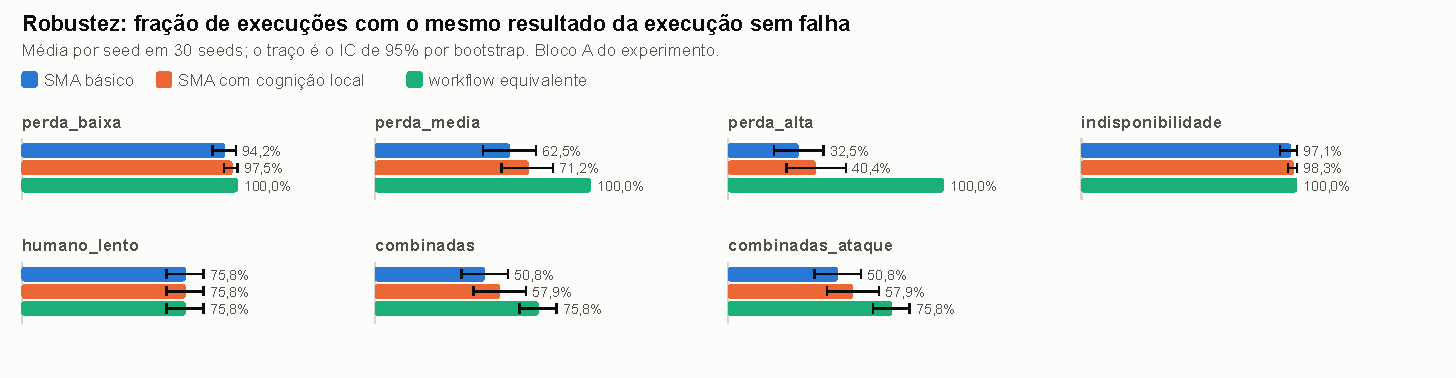
\includegraphics[width=\linewidth]{figuras/fig_robustez.pdf}
\caption{Robustez por condição, média por seed com IC de 95\% (gerada pelo comando do experimento a partir de
\code{execucoes.csv}).}\label{fig:robustez}
\end{figure}

\paragraph{RQ3 --- custo de coordenação e do controle de acesso.} Sem falhas, o SMA troca \V{rq3.nominal.msg.dif}
mensagens de coordenação a mais por solicitação \V{rq3.nominal.msg.dif.ic} e leva \V{rq3.nominal.lat.dif} ticks a mais
\V{rq3.nominal.lat.dif.ic}; sob falhas combinadas, \V{rq3.combinadas.lat.dif} ticks a mais \V{rq3.combinadas.lat.dif.ic};
todas com p ajustado $<$\,0,001 (Tabela~\ref{tab:rq3}, Figura~\ref{fig:custo}). Ligar o controle de acesso por pessoa não
mudou mensagens, latência nem registros do trace em nenhuma das \V{exp.seeds} seeds (\V{rq3.acesso.mensagens.pares},
\V{rq3.acesso.latencia_ticks.pares} e \V{rq3.acesso.registros_trace.pares} seeds diferentes): o atestado viaja dentro da
mensagem de aprovação. A previsão de mais registros de auditoria não se confirmou, porque o que o acesso registra a mais
vai para a trilha de acesso, outro arquivo, que não foi medido.

\begin{tabela}{RQ3, custo por solicitação (bloco A, média por seed).\label{tab:rq3}}
\begin{tabularx}{\linewidth}{Y R{1.9cm} R{1.9cm} R{1.9cm} R{1.9cm} R{1.9cm} R{1.9cm}}
\toprule
& \multicolumn{3}{c}{\textbf{Mensagens de coordenação}} & \multicolumn{3}{c}{\textbf{Latência (ticks)}}\\
\cmidrule(lr){2-4}\cmidrule(lr){5-7}
\textbf{Condição} & \textbf{SMA básico} & \textbf{SMA local} & \textbf{Workflow} & \textbf{SMA básico} & \textbf{SMA local} & \textbf{Workflow}\\ \midrule
\TabRQtres
\bottomrule
\end{tabularx}
\end{tabela}

\begin{figure}[tbp]\centering
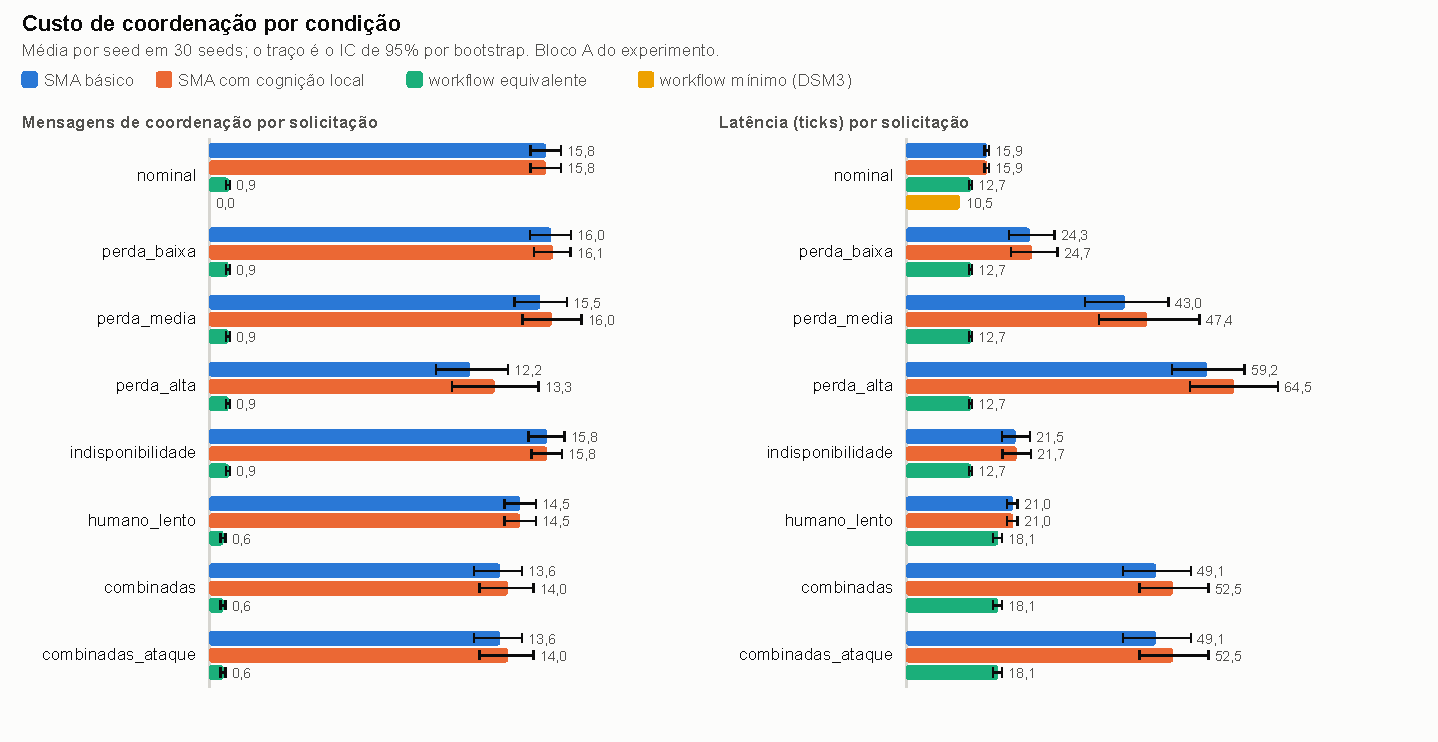
\includegraphics[width=0.92\linewidth]{figuras/fig_custo.pdf}
\caption{Custo de coordenação e latência por condição (o workflow mínimo só roda sem falhas).}\label{fig:custo}
\end{figure}

\paragraph{RQ4 --- recuperação.} Depois da correção, o SMA responde sempre: \V{exp.sem_resposta} execuções sem resposta
explícita. Responder não é acertar: a maior parte das execuções atingidas por 30\% de perda termina em falha explícita
(Tabela~\ref{tab:rq4}), porque o Orquestrador reenvia uma vez e, se perde de novo, responde \code{failure}. A
recuperação custa de \V{rq4.perda_baixa.mediana} a \V{rq4.perda_alta.mediana} ticks na mediana, bem acima de um prazo de
consulta. Recuperar de perda leva mais que de indisponibilidade (\V{rq4.tipo.a} contra \V{rq4.tipo.b} ticks em média; p
ajustado \V{rq4.tipo.p}, delta \V{rq4.tipo.cliff}).

\begin{tabela}{RQ4, SMA básico, execuções atingidas por pelo menos uma perda ou prazo esgotado (bloco A).\label{tab:rq4}}
\begin{tabularx}{\linewidth}{Y R{2.2cm} R{3.0cm} R{2.4cm} R{1.8cm} R{2.6cm}}
\toprule
\textbf{Condição} & \textbf{Atingidas} & \textbf{Mesmo resultado da nominal} & \textbf{Degradação segura} & \textbf{Sem resposta} & \textbf{Recuperação (mediana, ticks)}\\ \midrule
\TabRQquatro
\bottomrule
\end{tabularx}
\end{tabela}

\paragraph{RQ5 --- porte e parâmetros.} A microempresa classifica pior: \V{rq5.porte.micro.sma_basico.classificacao}
contra \V{rq5.porte.pequena.sma_basico.classificacao} na pequena (\V{rq5.porte.dif} \V{rq5.porte.dif.ic}, p ajustado
\V{rq5.porte.p}), em parte porque sem ERP não há segunda fonte para reconciliar quando a planilha diverge, em parte por
dois efeitos da geração de dados nesse porte (Seção~\ref{sec:ameacas}); o workflow tem os mesmos números em todos os
portes. Na varredura (Tabela~\ref{tab:rq5}), mais tentativas aumentam a robustez e a latência (p ajustado
\V{rq5.teste.tentativas.p}), prazo de subtarefa maior aumenta a latência (\V{rq5.teste.prazo_subtarefa.p}) e sem correção
não há crítica corrigida (\V{rq5.teste.correcoes.p}). Prazo de aprovação e TTL da reserva apontam no sentido previsto sem
significância (\V{rq5.teste.prazo_aprovacao.seeds} seeds diferentes cada); o limiar de 5\% não mudou nada e o de 20\%
derruba a classificação, mas perde a significância depois de Holm (p ajustado \V{rq5.teste.limiar20.p}).

\begin{tabela}{RQ5, varredura de parâmetros (bloco B, porte médio, SMA básico), na medida designada no pré-registro. Em negrito, o valor padrão.\label{tab:rq5}}
\begin{tabularx}{\linewidth}{L{3.0cm} L{2.0cm} L{3.8cm} Y}
\toprule
\textbf{Parâmetro} & \textbf{Condição} & \textbf{Medida} & \textbf{Nível: valor}\\ \midrule
\TabRQcinco
\bottomrule
\end{tabularx}
\end{tabela}

\paragraph{RQ6 --- ataques sob falha.}\label{sec:rq6} No bloco A, \V{rq6.A.ataques_tentados} ataques ao Approval Gate em
\V{rq6.A.execucoes_atacadas} execuções atacadas, com perda, atraso, indisponibilidade e humano lento ao mesmo tempo:
\V{rq6.A.ataques_aceitos} aceitos. No bloco D, com o controle de acesso ligado, \V{rq6.D.ataques_tentados} ataques:
\V{rq6.D.ataques_aceitos} registrados como aceitos, todos o mesmo ataque e nenhum indevido (\V{rq6.D.aceitos_indevidos}):
o ataque supõe que a analista participou do lançamento vetado, e com plantios sorteados isso nem sempre é verdade;
quando ela não participou, a decisão é a de uma aprovadora autorizada e a política a aceita corretamente. A execução
atacada terminou igual à mesma execução sem ataque em todos os \V{rq6.sma_basico.pares} pares do SMA básico e nos
\V{rq6.sma_local.pares} do SMA local. O workflow equivalente não foi atacado: a bateria é contra o barramento de
agentes, e o controlador único não tem as fronteiras que ela testa.

\paragraph{RQ7 --- cognição local.}\label{sec:rq7} Sem falhas, o braço local é idêntico ao básico
(\V{rq7.pares.diferentes} pares diferentes em \V{rq7.pares}), sem mensagem nem tick a mais; o custo aparece em decisões
registradas (\V{rq7.nominal.decisoes.local} contra \V{rq7.nominal.decisoes.basico} por solicitação) e em trace. Sob
perda, a classificação correta, que era a medida registrada, difere em poucas seeds e nenhum teste a distingue do acaso,
nem no subgrupo registrado (Tabela~\ref{tab:rq7}). Também não houve mais mensagens (\V{rq7.msg.dif} \V{rq7.msg.dif.ic},
p ajustado \V{rq7.msg.p}). \textbf{Na medida registrada, a cognição local não mostrou ganho.}

\begin{tabela}{RQ7, classificação correta, SMA básico $\times$ SMA local (bloco A; família RQ7, p ajustado por Holm; --- quando o resultado é idêntico em todos os pares e o teste não se aplica).\label{tab:rq7}}
\begin{tabularx}{\linewidth}{Y R{2.0cm} R{2.0cm} R{2.0cm} R{1.8cm}}
\toprule
\textbf{Condição} & \textbf{SMA básico} & \textbf{SMA local} & \textbf{Seeds dif.} & \textbf{p ajust.}\\ \midrule
\TabRQsete
\bottomrule
\end{tabularx}
\end{tabela}

Numa medida que não estava designada para RQ7 (execução correta), o braço local fica acima do básico em todas as
condições de falha de comunicação (Tabela~\ref{tab:rq7expl}). É exploratório: calculado depois de ver os dados, fora de
qualquer família de testes, sobre um braço cujo conteúdo mudou depois do pré-registro, e nenhuma diferença é
significativa nem antes de corrigir. O sinal é consistente no sentido e pequeno; o experimento não tem poder para
afirmá-lo, e mesmo com ele o braço local fica muito abaixo do workflow equivalente sob perda.

\begin{tabela}{Exploratório: execução correta, SMA local menos SMA básico (bloco A; p de Wilcoxon sem correção; recalculado de \code{execucoes.csv}).\label{tab:rq7expl}}
\begin{tabularx}{\linewidth}{Y R{2.0cm} R{2.0cm} R{3.6cm} R{1.6cm} R{1.5cm}}
\toprule
\textbf{Condição} & \textbf{SMA básico} & \textbf{SMA local} & \textbf{Diferença [IC 95\%]} & \textbf{Seeds dif.} & \textbf{p}\\ \midrule
\TabRQseteExpl
\bottomrule
\end{tabularx}
\end{tabela}

\paragraph{Ablação.}\label{sec:ablacao} Base: SMA local com tudo ligado, porte médio, desvio irregular sempre plantado e,
no fechamento, um segundo pedido do mesmo mês dois ticks depois (Tabela~\ref{tab:ablacao}, Figura~\ref{fig:ablacao}). Três
mecanismos têm contribuição clara. O \textbf{reenvio} do Orquestrador é o mecanismo de recuperação que funciona (na
primeira rodada, antes da correção, não se distinguia do acaso, porque não cobria a resposta perdida). A \textbf{reserva
de período} é a única coisa que impede dois fechamentos do mesmo mês: sem ela, os dois foram publicados em todas as
seeds. O \textbf{veto com correção}: sem ele, o aprovador diligente concede waiver e o cauteloso bloqueia, e a publicação
cai para \V{abl.sem_correcao.publicacao}. A \textbf{negociação de prazo} não mostrou efeito na medida designada, e a
\textbf{cognição local} aponta no sentido esperado sem significância.

\begin{tabela}{Ablação (bloco C): um mecanismo desligado por vez, na medida designada; p ajustado por Holm na família da ablação.\label{tab:ablacao}}
\begin{tabularx}{\linewidth}{L{3.4cm} Y R{1.8cm} R{1.8cm} R{1.5cm} R{1.6cm}}
\toprule
\textbf{Mecanismo desligado} & \textbf{Medida designada} & \textbf{Com} & \textbf{Sem} & \textbf{Seeds dif.} & \textbf{p ajust.}\\ \midrule
\TabAblacao
\bottomrule
\end{tabularx}
\end{tabela}

\begin{figure}[tbp]\centering
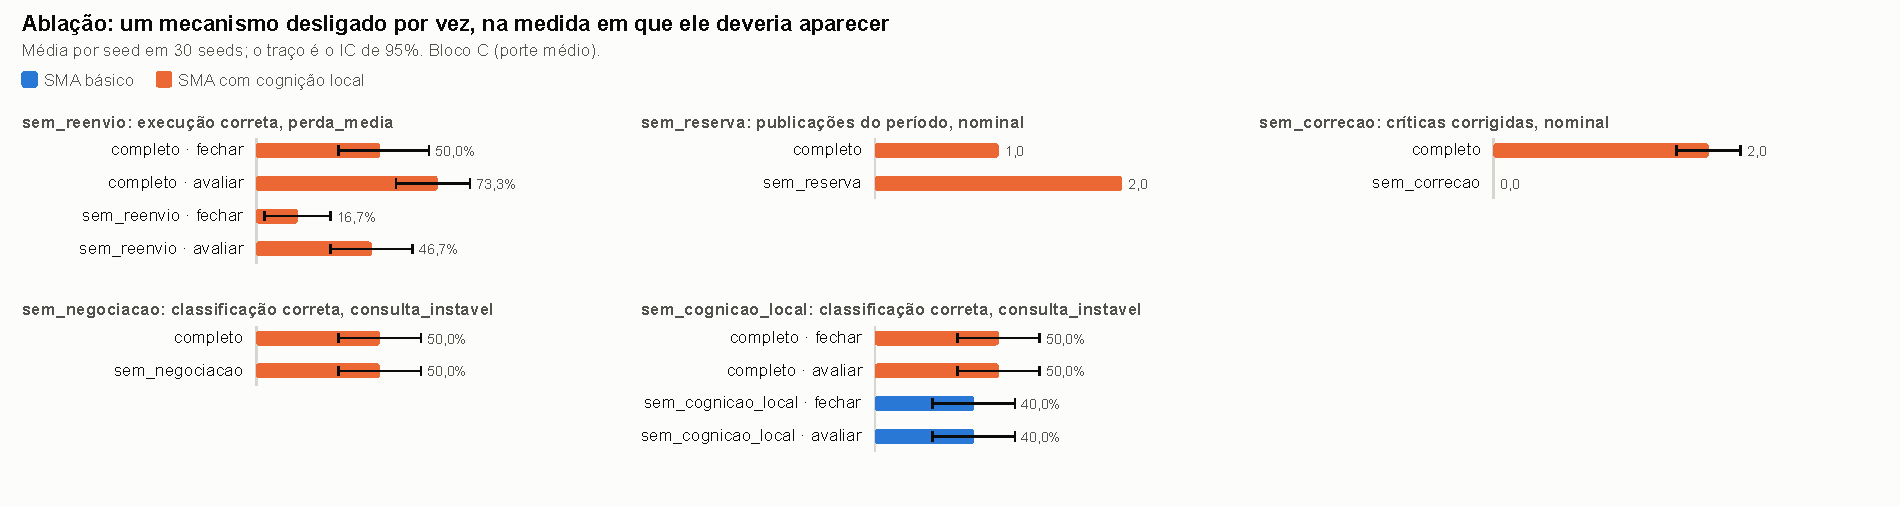
\includegraphics[width=\linewidth]{figuras/fig_ablacao.pdf}
\caption{Ablação: cada mecanismo desligado contra o sistema completo.}\label{fig:ablacao}
\end{figure}

\subsection{Duas rodadas}
O experimento rodou duas vezes, e as duas contam. A primeira (dados no commit \code{\V{r1.commit}}, CSV
\code{\V{r1.sha}\ldots}) mediu a v0.5.0 como estava e revelou o defeito da resposta perdida. O defeito foi corrigido e a
segunda rodada (commit \code{\V{r2.commit}}, CSV \code{\V{exp.sha}\ldots}) mede o sistema entregue. \textbf{A segunda
rodada não é teste confirmatório} das hipóteses de robustez e recuperação: o sistema mudou justamente onde a primeira
mostrou que falhava. Entre as rodadas mudaram três coisas, não uma: a correção (com ajustes no verificador de
invariantes), o lugar do sorteio do atraso de entrega (as condições com atraso não repetem as mesmas realizações) e o
conteúdo do braço local (na segunda, também AG-RES, AG-CUS e AG-REL são BDI). Para o SMA básico nas condições sem
atraso, a diferença entre as rodadas é atribuível à correção; nas outras, não dá para separar.

\begin{tabela}{As duas rodadas lado a lado (SMA básico, salvo indicação).\label{tab:rodadas}}
\begin{tabularx}{\linewidth}{Y L{3.8cm} L{3.6cm} L{2.2cm}}
\toprule
\textbf{Medida} & \textbf{Primeira rodada} & \textbf{Segunda rodada} & \textbf{Workflow equiv.}\\ \midrule
\TabDuasRodadas
\bottomrule
\end{tabularx}
\end{tabela}

O que a correção mudou: toda solicitação passou a ter resposta; a robustez do SMA subiu em todas as condições de falha
de comunicação; o reenvio passou a ter efeito; com 5\% de perda, a diferença para o workflow deixou de ser significativa.
O que não mudou, e por isso não depende da correção: \textbf{o empate de qualidade, o custo maior, a robustez menor que a
do workflow a partir de 15\% de perda, zero ataque aceito indevidamente e zero crítica publicada sem tratamento}. A
latência sob falha ficou maior, porque as execuções que antes travavam agora esperam o prazo, reenviam e entram na média.

\subsection{Comportamento coletivo observado}
Onde a distribuição custou: cada decisão local precisa de uma troca para ser conhecida pelos outros (mensagens); cada
troca pode se perder (exposição); recuperar leva de duas a quatro vezes uma solicitação inteira sem falha; e um reenvio
por subtarefa é pouco quando a perda é alta (\V{rq4.perda_alta.falhas} de \V{rq4.perda_alta.execucoes} execuções do SMA básico com 30\% de perda
terminam em degradação segura). Onde a distribuição ajudou: em nada que este experimento meça como resultado quando as
funções são iguais. Na contenção, os ataques vindos de identidades falsas, de agentes legítimos fora do papel e da
caixa do aprovador sem a pessoa certa foram todos rejeitados com o sistema degradado e nenhum mudou o desfecho; isso
depende de cada agente ter papel, credencial e lista de ferramentas próprios, coisa que o controlador único não tem para
ser atacada do mesmo modo. Na concorrência, a reserva de período, um mecanismo de coordenação, foi o que impediu a dupla
publicação. O que as falhas não quebraram: nenhuma crítica publicada sem tratamento nas \V{exp.sma.execucoes} execuções
do SMA, em nenhuma rodada, e nenhum invariante violado na segunda.

\subsection{O que não se confirmou}
\begin{enumerate}
  \item H7b e H7c: a cognição local não melhora a classificação de forma distinguível do acaso nem custa mais mensagens.
  \item H2a para 5\% de perda e para a indisponibilidade de um especialista: sinal previsto, sem significância.
  \item H4a para 30\% de perda e para as falhas combinadas: a maioria das atingidas não recupera o resultado.
  \item H5b para o limiar de 5\% (nenhum efeito), o de 20\% (não significativo após Holm), o prazo de aprovação e o TTL
        da reserva (não significativos).
  \item H3b na parte da auditoria: o trace não cresce com o controle de acesso.
  \item Ablação da negociação de prazo e da cognição local: contribuição não distinguível do acaso.
  \item A expectativa de zero violações, na primeira rodada: \V{r1.violacoes} execuções violaram o INV-07.
\end{enumerate}

\subsection{Desvios do pré-registro}
O pré-registro dizia que o defeito previsto seria medido, não corrigido; ele foi corrigido e o experimento rodou de
novo. O defeito era mais amplo que o previsto (estava também no PROT-DEL e respondia pela maior parte das execuções sem
resposta). O braço local mudou de conteúdo. O sorteio do atraso mudou de lugar. MEI e Média empresa II, que entraram
depois, ficaram fora (o workflow equivalente não implementa as regras deles). A métrica de ataques foi desdobrada em
bruto e sem a premissa do ataque, depois de ver o primeiro caso numa rodada de teste do aparato. Duas medidas são
exploratórias. Rodadas de fumaça do aparato foram olhadas antes (seeds 1 a 3 e uma configuração que não é condição do
experimento); seeds, condições, tamanho da amostra e comparações não mudaram. O bloco de fuzz citado no plano geral não
foi feito. A lista completa, com as reexecuções e suas causas, está em \code{docs/dsm4/resultados.md}.

\subsection{Ameaças à validade}\label{sec:ameacas}
\textbf{Construto.} A robustez favorece o workflow por construção: o modelo de falhas atinge a comunicação entre agentes,
e um workflow distribuído (controlador com serviços remotos) não foi construído. O que o SMA compra (separação de
autoridade, menor privilégio, trilha de quem decidiu) não aparece em métrica de resultado. Um tick é unidade do relógio
lógico, e os 3 ticks por etapa do workflow são premissa. O gabarito de classificação tem teto abaixo de 100\% em três
situações (desvio orçamentário e irregular na mesma conta; na micro, desvio plantado exatamente no limiar; na micro,
duplicidade descontada do desvio), que atingem SMA e workflow por igual. \textbf{Interna.} O workflow equivalente foi
escrito depois do SMA, pelos mesmos autores, lendo os agentes; a equivalência é testada só sem falhas. A segunda rodada foi
medida depois de corrigir o que a primeira mostrou. O pareamento entre SMA e workflow é parcial: os braços trocam mensagens
diferentes. \textbf{Externa.} Dados sintéticos com plantio; perda independente por mensagem, sem rajadas nem partição;
Orquestrador que não cai; um único nível de recuperação (um reenvio), escolha que determina boa parte da distância para
o workflow sob perda alta (com três tentativas, \V{rq5.max_tentativas.3} contra \V{rq5.max_tentativas.2} nas combinadas).
\textbf{Conclusão.} Como a perda é sorteada por mensagem com chave comum, as oito células de uma seed compartilham o
destino das mensagens: o efeito aparece em poucas seeds inteiras e as comparações de cognição e negociação têm pouco
poder. Holm controla o erro por família, não no experimento inteiro. A amostra não teve aprovador rigoroso (probabilidade
0,10; não saiu nas 30 seeds).

% ---------------------------------------------------------------- 11
\section{Limitações}
A lista completa e sem suavização está em \code{docs/dsm4/limitacoes.md}. As que mais pesam:
\begin{itemize}
  \item \textbf{O SMA não ganha do workflow equivalente em nenhuma métrica de resultado}, e perde em custo e em
        robustez sob perda de mensagens. A recuperação é um reenvio por subtarefa.
  \item \textbf{Raiz de confiança no processo e no disco}: credenciais em memória do processo; chaves simétricas na
        pasta de chaves; quem lê essa pasta forja trace, memória ou cadastro válidos. Barramento em processo, sem rede;
        numa versão distribuída, mTLS ou assinatura por mensagem.
  \item \textbf{Ponto único de falha}: o Orquestrador não cai no experimento nem tem substituto.
  \item \textbf{Cognição}: o pacote local não mostrou ganho; o AG-REL BDI não acrescenta capacidade; as regras locais
        reconhecem poucas formas de escrever; nenhum LLM real foi avaliado.
  \item \textbf{Pedido sem atestado}: a pessoa do pedido vem da sessão da interface, não de um atestado no PROT-SOL; a
        resposta final ao solicitante, se perdida, não é avisada.
  \item \textbf{Dados sintéticos}: o gabarito é o que foi plantado; empresas reais têm erros combinados e ambíguos.
  \item \textbf{Interfaces}: TUI não verificada em Windows; expiração de sessão por tempo sem teste automatizado; os
        roteiros Playwright não foram executados na geração deste relatório; delegações, empresa ativa, segundo fator
        e cofre não têm tela no dashboard web.
  \item \textbf{Cofre sem cifra}: integridade e controle de acesso, não confidencialidade contra quem lê o disco.
  \item \textbf{Fontes}: nenhum conector de fornecedor nem ERP real testado; o entendimento de fontes depende de um
        vocabulário finito de sinônimos, e o que ele não reconhece a pessoa mapeia à mão.
\end{itemize}
Saíram da lista da DSM3 nesta entrega: o experimento sem variância e desequilibrado, os especialistas só reativos, a
resposta perdida que virava silêncio, a senha como único fator, o aprovador sem limite de valor e sem substituto, a
memória que perdia entradas entre processos e o cadastro de uma empresa só.
% Integrado da branch dsm4/v1.0.0 (ADR-011 e ADR-012).

% ---------------------------------------------------------------- 12
\section{Conclusão}
Para este problema e este tamanho, um controlador centralizado com as mesmas regras entrega a mesma qualidade, com menos
mensagens e sem a exposição à perda de mensagens. O SMA não se justifica pelo resultado medido, e o relatório não
transforma isso em empate técnico. O que a arquitetura de agentes entrega e o workflow não entrega são propriedades de
desenho, verificáveis por teste e por trace, mas não por métricas de resultado: \textbf{separação de responsabilidades
auditável} (quem calcula não julga conformidade, quem julga não aprova, e cada decisão tem autor no trace);
\textbf{veto independente} do AG-CIN, que nenhum outro agente consegue contornar; \textbf{decisão humana atestada} pela
pessoa autenticada, com cargo e segregação de funções conferidos; \textbf{negociação} explícita de prazo entre quem
executa e quem coordena; e \textbf{extensibilidade} (um especialista novo entra com papel, protocolos e allowlist
próprios, sem tocar nos demais). O experimento mostrou que essas garantias se mantêm com o sistema degradado (zero
crítica publicada sem tratamento, zero ataque aceito indevidamente) e mostrou também onde a distribuição custa. Os
trabalhos seguintes que os dados indicam são uma recuperação mais forte que um reenvio, um workflow distribuído como
linha de base justa para robustez e a medição de um modelo real na bancada de hipóteses, fora do experimento principal.

% ---------------------------------------------------------------- apêndice
\clearpage
\appendix
\section{Grafos de rastreabilidade por parte}\label{ap:trace}
Gerados de \code{models/*.yaml} por \code{tools/relatorio\_numeros.py} (as mesmas cadeias que o \code{tools/trace.py
-{}-check} valida e que a documentação navegável mostra por \code{needflow}). O número de testes é o de testes modelados
que verificam o requisito.

% Gerado por tools/relatorio_numeros.py; não edite à mão.
\begin{figure}[H]\centering
\begin{tikzpicture}[font=\sffamily\scriptsize, >={Stealth[length=1.6mm]},
 caixa/.style={draw=black!45, rounded corners=1.5pt, align=left, inner sep=2.5pt, anchor=north west}]
\node[anchor=south west, inner sep=0pt, font=\sffamily\scriptsize\bfseries] at (0.0,0.15) {Requisito};
\node[anchor=south west, inner sep=0pt, font=\sffamily\scriptsize\bfseries] at (4.0,0.15) {Papéis};
\node[anchor=south west, inner sep=0pt, font=\sffamily\scriptsize\bfseries] at (7.5,0.15) {Protocolos e normas};
\node[anchor=south west, inner sep=0pt, font=\sffamily\scriptsize\bfseries] at (11.8,0.15) {Testes};
\node[anchor=south west, inner sep=0pt, font=\sffamily\scriptsize\bfseries] at (13.9,0.15) {Métricas};
\node[caixa, fill=trreq, text width=3.45cm] (c0r8) at (0.0,-0.00) {\textbf{REQ-F01} (DSM1)\\Decomposição e agregação de solicitações};
\node[caixa, fill=trpapel, text width=2.95cm] (c1r9) at (4.0,-0.00) {ROLE-ORQ, ROLE-SOL};
\node[caixa, fill=trprot, text width=3.75cm] (c2r10) at (7.5,-0.00) {PROT-SOL, PROT-DEL};
\node[caixa, fill=trteste, text width=1.55cm] (c3r11) at (11.8,-0.00) {22 teste(s)};
\node[caixa, fill=trmet, text width=3.35cm] (c4r12) at (13.9,-0.00) {MET-01, MET-04, MET-09, MET-13, MET-41, MET-42, MET-43, MET-47};
\draw[->, black!55] ([yshift=-0.22cm]c0r8.north east) -- ([yshift=-0.22cm]c0r8.north east -| c1r9.west);
\draw[->, black!55] ([yshift=-0.22cm]c1r9.north east) -- ([yshift=-0.22cm]c1r9.north east -| c2r10.west);
\draw[->, black!55] ([yshift=-0.22cm]c2r10.north east) -- ([yshift=-0.22cm]c2r10.north east -| c3r11.west);
\draw[->, black!55] ([yshift=-0.22cm]c3r11.north east) -- ([yshift=-0.22cm]c3r11.north east -| c4r12.west);
\node[caixa, fill=trreq, text width=3.45cm] (c0r17) at (0.0,-1.34) {\textbf{REQ-F02} (DSM1)\\Apuração de custos, margem e rentabilidade};
\node[caixa, fill=trpapel, text width=2.95cm] (c1r18) at (4.0,-1.34) {ROLE-CUS};
\node[caixa, fill=trprot, text width=3.75cm] (c2r19) at (7.5,-1.34) {PROT-DEL};
\node[caixa, fill=trteste, text width=1.55cm] (c3r20) at (11.8,-1.34) {6 teste(s)};
\node[caixa, fill=trmet, text width=3.35cm] (c4r21) at (13.9,-1.34) {MET-02};
\draw[->, black!55] ([yshift=-0.22cm]c0r17.north east) -- ([yshift=-0.22cm]c0r17.north east -| c1r18.west);
\draw[->, black!55] ([yshift=-0.22cm]c1r18.north east) -- ([yshift=-0.22cm]c1r18.north east -| c2r19.west);
\draw[->, black!55] ([yshift=-0.22cm]c2r19.north east) -- ([yshift=-0.22cm]c2r19.north east -| c3r20.west);
\draw[->, black!55] ([yshift=-0.22cm]c3r20.north east) -- ([yshift=-0.22cm]c3r20.north east -| c4r21.west);
\node[caixa, fill=trreq, text width=3.45cm] (c0r26) at (0.0,-2.68) {\textbf{REQ-F03} (DSM1)\\Orçado x realizado e forecast};
\node[caixa, fill=trpapel, text width=2.95cm] (c1r27) at (4.0,-2.68) {ROLE-ORC};
\node[caixa, fill=trprot, text width=3.75cm] (c2r28) at (7.5,-2.68) {PROT-DEL, PROT-QRY};
\node[caixa, fill=trteste, text width=1.55cm] (c3r29) at (11.8,-2.68) {12 teste(s)};
\node[caixa, fill=trmet, text width=3.35cm] (c4r30) at (13.9,-2.68) {MET-02, MET-14, MET-44};
\draw[->, black!55] ([yshift=-0.22cm]c0r26.north east) -- ([yshift=-0.22cm]c0r26.north east -| c1r27.west);
\draw[->, black!55] ([yshift=-0.22cm]c1r27.north east) -- ([yshift=-0.22cm]c1r27.north east -| c2r28.west);
\draw[->, black!55] ([yshift=-0.22cm]c2r28.north east) -- ([yshift=-0.22cm]c2r28.north east -| c3r29.west);
\draw[->, black!55] ([yshift=-0.22cm]c3r29.north east) -- ([yshift=-0.22cm]c3r29.north east -| c4r30.west);
\node[caixa, fill=trreq, text width=3.45cm] (c0r35) at (0.0,-4.02) {\textbf{REQ-F04} (DSM1)\\Resultado consolidado via A2A};
\node[caixa, fill=trpapel, text width=2.95cm] (c1r36) at (4.0,-4.02) {ROLE-RES, ROLE-CUS, ROLE-ORC};
\node[caixa, fill=trprot, text width=3.75cm] (c2r37) at (7.5,-4.02) {PROT-QRY, PROT-DEL};
\node[caixa, fill=trteste, text width=1.55cm] (c3r38) at (11.8,-4.02) {7 teste(s)};
\node[caixa, fill=trmet, text width=3.35cm] (c4r39) at (13.9,-4.02) {MET-02, MET-04, MET-43};
\draw[->, black!55] ([yshift=-0.22cm]c0r35.north east) -- ([yshift=-0.22cm]c0r35.north east -| c1r36.west);
\draw[->, black!55] ([yshift=-0.22cm]c1r36.north east) -- ([yshift=-0.22cm]c1r36.north east -| c2r37.west);
\draw[->, black!55] ([yshift=-0.22cm]c2r37.north east) -- ([yshift=-0.22cm]c2r37.north east -| c3r38.west);
\draw[->, black!55] ([yshift=-0.22cm]c3r38.north east) -- ([yshift=-0.22cm]c3r38.north east -| c4r39.west);
\end{tikzpicture}
\caption{Rastreabilidade, funcional: REQ-F01 a REQ-F04. Cadeia requisito $\rightarrow$ papéis $\rightarrow$ protocolos e normas $\rightarrow$ testes $\rightarrow$ métricas, lida de \texttt{models/*.yaml}.}
\label{fig:trace1}
\end{figure}

\begin{figure}[H]\centering
\begin{tikzpicture}[font=\sffamily\scriptsize, >={Stealth[length=1.6mm]},
 caixa/.style={draw=black!45, rounded corners=1.5pt, align=left, inner sep=2.5pt, anchor=north west}]
\node[anchor=south west, inner sep=0pt, font=\sffamily\scriptsize\bfseries] at (0.0,0.15) {Requisito};
\node[anchor=south west, inner sep=0pt, font=\sffamily\scriptsize\bfseries] at (4.0,0.15) {Papéis};
\node[anchor=south west, inner sep=0pt, font=\sffamily\scriptsize\bfseries] at (7.5,0.15) {Protocolos e normas};
\node[anchor=south west, inner sep=0pt, font=\sffamily\scriptsize\bfseries] at (11.8,0.15) {Testes};
\node[anchor=south west, inner sep=0pt, font=\sffamily\scriptsize\bfseries] at (13.9,0.15) {Métricas};
\node[caixa, fill=trreq, text width=3.45cm] (c0r8) at (0.0,-0.00) {\textbf{REQ-F05} (DSM1)\\Controles internos com veto};
\node[caixa, fill=trpapel, text width=2.95cm] (c1r9) at (4.0,-0.00) {ROLE-CIN, ROLE-ORQ};
\node[caixa, fill=trprot, text width=3.75cm] (c2r10) at (7.5,-0.00) {PROT-CMP, NORM-04};
\node[caixa, fill=trteste, text width=1.55cm] (c3r11) at (11.8,-0.00) {22 teste(s)};
\node[caixa, fill=trmet, text width=3.35cm] (c4r12) at (13.9,-0.00) {MET-03, MET-14, MET-44};
\draw[->, black!55] ([yshift=-0.22cm]c0r8.north east) -- ([yshift=-0.22cm]c0r8.north east -| c1r9.west);
\draw[->, black!55] ([yshift=-0.22cm]c1r9.north east) -- ([yshift=-0.22cm]c1r9.north east -| c2r10.west);
\draw[->, black!55] ([yshift=-0.22cm]c2r10.north east) -- ([yshift=-0.22cm]c2r10.north east -| c3r11.west);
\draw[->, black!55] ([yshift=-0.22cm]c3r11.north east) -- ([yshift=-0.22cm]c3r11.north east -| c4r12.west);
\node[caixa, fill=trreq, text width=3.45cm] (c0r17) at (0.0,-1.34) {\textbf{REQ-F06} (DSM1)\\Relatório executivo por template com LLM opcional};
\node[caixa, fill=trpapel, text width=2.95cm] (c1r18) at (4.0,-1.34) {ROLE-REL};
\node[caixa, fill=trprot, text width=3.75cm] (c2r19) at (7.5,-1.34) {PROT-DEL, NORM-05, NORM-07};
\node[caixa, fill=trteste, text width=1.55cm] (c3r20) at (11.8,-1.34) {6 teste(s)};
\node[caixa, fill=trmet, text width=3.35cm] (c4r21) at (13.9,-1.34) {MET-06};
\draw[->, black!55] ([yshift=-0.22cm]c0r17.north east) -- ([yshift=-0.22cm]c0r17.north east -| c1r18.west);
\draw[->, black!55] ([yshift=-0.22cm]c1r18.north east) -- ([yshift=-0.22cm]c1r18.north east -| c2r19.west);
\draw[->, black!55] ([yshift=-0.22cm]c2r19.north east) -- ([yshift=-0.22cm]c2r19.north east -| c3r20.west);
\draw[->, black!55] ([yshift=-0.22cm]c3r20.north east) -- ([yshift=-0.22cm]c3r20.north east -| c4r21.west);
\node[caixa, fill=trreq, text width=3.45cm] (c0r26) at (0.0,-3.02) {\textbf{REQ-F07} (DSM1)\\Memória de longo prazo com proveniência};
\node[caixa, fill=trpapel, text width=2.95cm] (c1r27) at (4.0,-3.02) {ROLE-CUS, ROLE-ORC, ROLE-RES, ROLE-REL};
\node[caixa, fill=trprot, text width=3.75cm] (c2r28) at (7.5,-3.02) {PROT-APR, NORM-08};
\node[caixa, fill=trteste, text width=1.55cm] (c3r29) at (11.8,-3.02) {13 teste(s)};
\node[caixa, fill=trmet, text width=3.35cm] (c4r30) at (13.9,-3.02) {MET-10};
\draw[->, black!55] ([yshift=-0.22cm]c0r26.north east) -- ([yshift=-0.22cm]c0r26.north east -| c1r27.west);
\draw[->, black!55] ([yshift=-0.22cm]c1r27.north east) -- ([yshift=-0.22cm]c1r27.north east -| c2r28.west);
\draw[->, black!55] ([yshift=-0.22cm]c2r28.north east) -- ([yshift=-0.22cm]c2r28.north east -| c3r29.west);
\draw[->, black!55] ([yshift=-0.22cm]c3r29.north east) -- ([yshift=-0.22cm]c3r29.north east -| c4r30.west);
\node[caixa, fill=trreq, text width=3.45cm] (c0r35) at (0.0,-4.36) {\textbf{REQ-F08} (DSM3)\\Cognição assistida por hipóteses verificáveis (local e LLM opcional)};
\node[caixa, fill=trpapel, text width=2.95cm] (c1r36) at (4.0,-4.36) {ROLE-ORC};
\node[caixa, fill=trprot, text width=3.75cm] (c2r37) at (7.5,-4.36) {PROT-QRY, PROT-DEL, NORM-05, NORM-07, NORM-11};
\node[caixa, fill=trteste, text width=1.55cm] (c3r38) at (11.8,-4.36) {10 teste(s)};
\node[caixa, fill=trmet, text width=3.35cm] (c4r39) at (13.9,-4.36) {MET-18, MET-45};
\draw[->, black!55] ([yshift=-0.22cm]c0r35.north east) -- ([yshift=-0.22cm]c0r35.north east -| c1r36.west);
\draw[->, black!55] ([yshift=-0.22cm]c1r36.north east) -- ([yshift=-0.22cm]c1r36.north east -| c2r37.west);
\draw[->, black!55] ([yshift=-0.22cm]c2r37.north east) -- ([yshift=-0.22cm]c2r37.north east -| c3r38.west);
\draw[->, black!55] ([yshift=-0.22cm]c3r38.north east) -- ([yshift=-0.22cm]c3r38.north east -| c4r39.west);
\end{tikzpicture}
\caption{Rastreabilidade, funcional: REQ-F05 a REQ-F08. Cadeia requisito $\rightarrow$ papéis $\rightarrow$ protocolos e normas $\rightarrow$ testes $\rightarrow$ métricas, lida de \texttt{models/*.yaml}.}
\label{fig:trace2}
\end{figure}

\begin{figure}[H]\centering
\begin{tikzpicture}[font=\sffamily\scriptsize, >={Stealth[length=1.6mm]},
 caixa/.style={draw=black!45, rounded corners=1.5pt, align=left, inner sep=2.5pt, anchor=north west}]
\node[anchor=south west, inner sep=0pt, font=\sffamily\scriptsize\bfseries] at (0.0,0.15) {Requisito};
\node[anchor=south west, inner sep=0pt, font=\sffamily\scriptsize\bfseries] at (4.0,0.15) {Papéis};
\node[anchor=south west, inner sep=0pt, font=\sffamily\scriptsize\bfseries] at (7.5,0.15) {Protocolos e normas};
\node[anchor=south west, inner sep=0pt, font=\sffamily\scriptsize\bfseries] at (11.8,0.15) {Testes};
\node[anchor=south west, inner sep=0pt, font=\sffamily\scriptsize\bfseries] at (13.9,0.15) {Métricas};
\node[caixa, fill=trreq, text width=3.45cm] (c0r8) at (0.0,-0.00) {\textbf{REQ-F20} (DSM4)\\Especialistas de Resultados, Custos e Relatórios com deliberação BDI};
\node[caixa, fill=trpapel, text width=2.95cm] (c1r9) at (4.0,-0.00) {ROLE-RES, ROLE-CUS, ROLE-REL, ROLE-ORC};
\node[caixa, fill=trprot, text width=3.75cm] (c2r10) at (7.5,-0.00) {PROT-DEL, PROT-QRY, NORM-07, NORM-08, NORM-11, NORM-20};
\node[caixa, fill=trteste, text width=1.55cm] (c3r11) at (11.8,-0.00) {27 teste(s)};
\node[caixa, fill=trmet, text width=3.35cm] (c4r12) at (13.9,-0.00) {MET-30};
\draw[->, black!55] ([yshift=-0.22cm]c0r8.north east) -- ([yshift=-0.22cm]c0r8.north east -| c1r9.west);
\draw[->, black!55] ([yshift=-0.22cm]c1r9.north east) -- ([yshift=-0.22cm]c1r9.north east -| c2r10.west);
\draw[->, black!55] ([yshift=-0.22cm]c2r10.north east) -- ([yshift=-0.22cm]c2r10.north east -| c3r11.west);
\draw[->, black!55] ([yshift=-0.22cm]c3r11.north east) -- ([yshift=-0.22cm]c3r11.north east -| c4r12.west);
\node[caixa, fill=trreq, text width=3.45cm] (c0r17) at (0.0,-2.02) {\textbf{REQ-F21} (DSM4)\\Conhecimento normativo com proveniência};
\node[caixa, fill=trpapel, text width=2.95cm] (c1r18) at (4.0,-2.02) {ROLE-CIN, ROLE-REL};
\node[caixa, fill=trprot, text width=3.75cm] (c2r19) at (7.5,-2.02) {PROT-CMP, NORM-02, NORM-21};
\node[caixa, fill=trteste, text width=1.55cm] (c3r20) at (11.8,-2.02) {6 teste(s)};
\node[caixa, fill=trmet, text width=3.35cm] (c4r21) at (13.9,-2.02) {MET-31};
\draw[->, black!55] ([yshift=-0.22cm]c0r17.north east) -- ([yshift=-0.22cm]c0r17.north east -| c1r18.west);
\draw[->, black!55] ([yshift=-0.22cm]c1r18.north east) -- ([yshift=-0.22cm]c1r18.north east -| c2r19.west);
\draw[->, black!55] ([yshift=-0.22cm]c2r19.north east) -- ([yshift=-0.22cm]c2r19.north east -| c3r20.west);
\draw[->, black!55] ([yshift=-0.22cm]c3r20.north east) -- ([yshift=-0.22cm]c3r20.north east -| c4r21.west);
\node[caixa, fill=trreq, text width=3.45cm] (c0r26) at (0.0,-3.36) {\textbf{REQ-F30} (DSM4)\\Fonte de dados por conector genérico e entendimento automático sem IA generativa};
\node[caixa, fill=trpapel, text width=2.95cm] (c1r27) at (4.0,-3.36) {ROLE-OPE, ROLE-ORQ};
\node[caixa, fill=trprot, text width=3.75cm] (c2r28) at (7.5,-3.36) {PROT-DEL, NORM-02, NORM-30, NORM-31};
\node[caixa, fill=trteste, text width=1.55cm] (c3r29) at (11.8,-3.36) {14 teste(s)};
\node[caixa, fill=trmet, text width=3.35cm] (c4r30) at (13.9,-3.36) {MET-50};
\draw[->, black!55] ([yshift=-0.22cm]c0r26.north east) -- ([yshift=-0.22cm]c0r26.north east -| c1r27.west);
\draw[->, black!55] ([yshift=-0.22cm]c1r27.north east) -- ([yshift=-0.22cm]c1r27.north east -| c2r28.west);
\draw[->, black!55] ([yshift=-0.22cm]c2r28.north east) -- ([yshift=-0.22cm]c2r28.north east -| c3r29.west);
\draw[->, black!55] ([yshift=-0.22cm]c3r29.north east) -- ([yshift=-0.22cm]c3r29.north east -| c4r30.west);
\end{tikzpicture}
\caption{Rastreabilidade, funcional: REQ-F20 a REQ-F30. Cadeia requisito $\rightarrow$ papéis $\rightarrow$ protocolos e normas $\rightarrow$ testes $\rightarrow$ métricas, lida de \texttt{models/*.yaml}.}
\label{fig:trace3}
\end{figure}

\begin{figure}[H]\centering
\begin{tikzpicture}[font=\sffamily\scriptsize, >={Stealth[length=1.6mm]},
 caixa/.style={draw=black!45, rounded corners=1.5pt, align=left, inner sep=2.5pt, anchor=north west}]
\node[anchor=south west, inner sep=0pt, font=\sffamily\scriptsize\bfseries] at (0.0,0.15) {Requisito};
\node[anchor=south west, inner sep=0pt, font=\sffamily\scriptsize\bfseries] at (4.0,0.15) {Papéis};
\node[anchor=south west, inner sep=0pt, font=\sffamily\scriptsize\bfseries] at (7.5,0.15) {Protocolos e normas};
\node[anchor=south west, inner sep=0pt, font=\sffamily\scriptsize\bfseries] at (11.8,0.15) {Testes};
\node[anchor=south west, inner sep=0pt, font=\sffamily\scriptsize\bfseries] at (13.9,0.15) {Métricas};
\node[caixa, fill=trreq, text width=3.45cm] (c0r8) at (0.0,-0.00) {\textbf{REQ-S01} (DSM1)\\Ações com efeito externo só com aprovação};
\node[caixa, fill=trpapel, text width=2.95cm] (c1r9) at (4.0,-0.00) {ROLE-ORQ, ROLE-REL, ROLE-ORC, ROLE-APR};
\node[caixa, fill=trprot, text width=3.75cm] (c2r10) at (7.5,-0.00) {PROT-APR, NORM-01, NORM-02, NORM-10};
\node[caixa, fill=trteste, text width=1.55cm] (c3r11) at (11.8,-0.00) {23 teste(s)};
\node[caixa, fill=trmet, text width=3.35cm] (c4r12) at (13.9,-0.00) {MET-05, MET-16};
\draw[->, black!55] ([yshift=-0.22cm]c0r8.north east) -- ([yshift=-0.22cm]c0r8.north east -| c1r9.west);
\draw[->, black!55] ([yshift=-0.22cm]c1r9.north east) -- ([yshift=-0.22cm]c1r9.north east -| c2r10.west);
\draw[->, black!55] ([yshift=-0.22cm]c2r10.north east) -- ([yshift=-0.22cm]c2r10.north east -| c3r11.west);
\draw[->, black!55] ([yshift=-0.22cm]c3r11.north east) -- ([yshift=-0.22cm]c3r11.north east -| c4r12.west);
\node[caixa, fill=trreq, text width=3.45cm] (c0r17) at (0.0,-1.34) {\textbf{REQ-S04} (DSM3)\\Autenticidade e integridade das interações (feedback da DSM2)};
\node[caixa, fill=trpapel, text width=2.95cm] (c1r18) at (4.0,-1.34) {ROLE-ORQ, ROLE-APR, ROLE-CIN, ROLE-SOL};
\node[caixa, fill=trprot, text width=3.75cm] (c2r19) at (7.5,-1.34) {PROT-SOL, PROT-DEL, PROT-QRY, PROT-CMP, PROT-APR, NORM-09, NORM-10};
\node[caixa, fill=trteste, text width=1.55cm] (c3r20) at (11.8,-1.34) {39 teste(s)};
\node[caixa, fill=trmet, text width=3.35cm] (c4r21) at (13.9,-1.34) {MET-15, MET-46};
\draw[->, black!55] ([yshift=-0.22cm]c0r17.north east) -- ([yshift=-0.22cm]c0r17.north east -| c1r18.west);
\draw[->, black!55] ([yshift=-0.22cm]c1r18.north east) -- ([yshift=-0.22cm]c1r18.north east -| c2r19.west);
\draw[->, black!55] ([yshift=-0.22cm]c2r19.north east) -- ([yshift=-0.22cm]c2r19.north east -| c3r20.west);
\draw[->, black!55] ([yshift=-0.22cm]c3r20.north east) -- ([yshift=-0.22cm]c3r20.north east -| c4r21.west);
\node[caixa, fill=trreq, text width=3.45cm] (c0r26) at (0.0,-3.02) {\textbf{REQ-S02} (DSM1)\\Exclusão mútua do período em fechamento};
\node[caixa, fill=trpapel, text width=2.95cm] (c1r27) at (4.0,-3.02) {ROLE-ORQ};
\node[caixa, fill=trprot, text width=3.75cm] (c2r28) at (7.5,-3.02) {PROT-LCK, NORM-03};
\node[caixa, fill=trteste, text width=1.55cm] (c3r29) at (11.8,-3.02) {11 teste(s)};
\node[caixa, fill=trmet, text width=3.35cm] (c4r30) at (13.9,-3.02) {MET-05};
\draw[->, black!55] ([yshift=-0.22cm]c0r26.north east) -- ([yshift=-0.22cm]c0r26.north east -| c1r27.west);
\draw[->, black!55] ([yshift=-0.22cm]c1r27.north east) -- ([yshift=-0.22cm]c1r27.north east -| c2r28.west);
\draw[->, black!55] ([yshift=-0.22cm]c2r28.north east) -- ([yshift=-0.22cm]c2r28.north east -| c3r29.west);
\draw[->, black!55] ([yshift=-0.22cm]c3r29.north east) -- ([yshift=-0.22cm]c3r29.north east -| c4r30.west);
\node[caixa, fill=trreq, text width=3.45cm] (c0r35) at (0.0,-4.36) {\textbf{REQ-S03} (DSM1)\\LLM não calcula nem autoriza};
\node[caixa, fill=trpapel, text width=2.95cm] (c1r36) at (4.0,-4.36) {ROLE-REL, ROLE-RES, ROLE-ORC};
\node[caixa, fill=trprot, text width=3.75cm] (c2r37) at (7.5,-4.36) {PROT-APR, NORM-05};
\node[caixa, fill=trteste, text width=1.55cm] (c3r38) at (11.8,-4.36) {8 teste(s)};
\node[caixa, fill=trmet, text width=3.35cm] (c4r39) at (13.9,-4.36) {MET-06};
\draw[->, black!55] ([yshift=-0.22cm]c0r35.north east) -- ([yshift=-0.22cm]c0r35.north east -| c1r36.west);
\draw[->, black!55] ([yshift=-0.22cm]c1r36.north east) -- ([yshift=-0.22cm]c1r36.north east -| c2r37.west);
\draw[->, black!55] ([yshift=-0.22cm]c2r37.north east) -- ([yshift=-0.22cm]c2r37.north east -| c3r38.west);
\draw[->, black!55] ([yshift=-0.22cm]c3r38.north east) -- ([yshift=-0.22cm]c3r38.north east -| c4r39.west);
\end{tikzpicture}
\caption{Rastreabilidade, segurança: REQ-S01 a REQ-S03. Cadeia requisito $\rightarrow$ papéis $\rightarrow$ protocolos e normas $\rightarrow$ testes $\rightarrow$ métricas, lida de \texttt{models/*.yaml}.}
\label{fig:trace4}
\end{figure}

\begin{figure}[H]\centering
\begin{tikzpicture}[font=\sffamily\scriptsize, >={Stealth[length=1.6mm]},
 caixa/.style={draw=black!45, rounded corners=1.5pt, align=left, inner sep=2.5pt, anchor=north west}]
\node[anchor=south west, inner sep=0pt, font=\sffamily\scriptsize\bfseries] at (0.0,0.15) {Requisito};
\node[anchor=south west, inner sep=0pt, font=\sffamily\scriptsize\bfseries] at (4.0,0.15) {Papéis};
\node[anchor=south west, inner sep=0pt, font=\sffamily\scriptsize\bfseries] at (7.5,0.15) {Protocolos e normas};
\node[anchor=south west, inner sep=0pt, font=\sffamily\scriptsize\bfseries] at (11.8,0.15) {Testes};
\node[anchor=south west, inner sep=0pt, font=\sffamily\scriptsize\bfseries] at (13.9,0.15) {Métricas};
\node[caixa, fill=trreq, text width=3.45cm] (c0r8) at (0.0,-0.00) {\textbf{REQ-S05} (DSM3)\\Identidade, sessão e autorização por pessoa};
\node[caixa, fill=trpapel, text width=2.95cm] (c1r9) at (4.0,-0.00) {ROLE-ADM, ROLE-APR, ROLE-OPE, ROLE-AUD, ROLE-SOL};
\node[caixa, fill=trprot, text width=3.75cm] (c2r10) at (7.5,-0.00) {PROT-APR, NORM-10, NORM-12, NORM-13};
\node[caixa, fill=trteste, text width=1.55cm] (c3r11) at (11.8,-0.00) {34 teste(s)};
\node[caixa, fill=trmet, text width=3.35cm] (c4r12) at (13.9,-0.00) {MET-17, MET-46};
\draw[->, black!55] ([yshift=-0.22cm]c0r8.north east) -- ([yshift=-0.22cm]c0r8.north east -| c1r9.west);
\draw[->, black!55] ([yshift=-0.22cm]c1r9.north east) -- ([yshift=-0.22cm]c1r9.north east -| c2r10.west);
\draw[->, black!55] ([yshift=-0.22cm]c2r10.north east) -- ([yshift=-0.22cm]c2r10.north east -| c3r11.west);
\draw[->, black!55] ([yshift=-0.22cm]c3r11.north east) -- ([yshift=-0.22cm]c3r11.north east -| c4r12.west);
\node[caixa, fill=trreq, text width=3.45cm] (c0r17) at (0.0,-1.68) {\textbf{REQ-S06} (DSM4)\\Acesso avançado — segundo fator, alçada por pessoa, delegação, quatro olhos, cofre e empresas};
\node[caixa, fill=trpapel, text width=2.95cm] (c1r18) at (4.0,-1.68) {ROLE-ADM, ROLE-APR};
\node[caixa, fill=trprot, text width=3.75cm] (c2r19) at (7.5,-1.68) {PROT-APR, PROT-CMP, NORM-14, NORM-15};
\node[caixa, fill=trteste, text width=1.55cm] (c3r20) at (11.8,-1.68) {48 teste(s)};
\node[caixa, fill=trmet, text width=3.35cm] (c4r21) at (13.9,-1.68) {MET-19};
\draw[->, black!55] ([yshift=-0.22cm]c0r17.north east) -- ([yshift=-0.22cm]c0r17.north east -| c1r18.west);
\draw[->, black!55] ([yshift=-0.22cm]c1r18.north east) -- ([yshift=-0.22cm]c1r18.north east -| c2r19.west);
\draw[->, black!55] ([yshift=-0.22cm]c2r19.north east) -- ([yshift=-0.22cm]c2r19.north east -| c3r20.west);
\draw[->, black!55] ([yshift=-0.22cm]c3r20.north east) -- ([yshift=-0.22cm]c3r20.north east -| c4r21.west);
\node[caixa, fill=trreq, text width=3.45cm] (c0r26) at (0.0,-4.04) {\textbf{REQ-S20} (DSM4)\\Credencial de conector selada e rede só em loopback salvo liberação do administrador};
\node[caixa, fill=trpapel, text width=2.95cm] (c1r27) at (4.0,-4.04) {ROLE-ADM, ROLE-OPE};
\node[caixa, fill=trprot, text width=3.75cm] (c2r28) at (7.5,-4.04) {PROT-APR, NORM-06, NORM-12, NORM-32};
\node[caixa, fill=trteste, text width=1.55cm] (c3r29) at (11.8,-4.04) {9 teste(s)};
\node[caixa, fill=trmet, text width=3.35cm] (c4r30) at (13.9,-4.04) {MET-50};
\draw[->, black!55] ([yshift=-0.22cm]c0r26.north east) -- ([yshift=-0.22cm]c0r26.north east -| c1r27.west);
\draw[->, black!55] ([yshift=-0.22cm]c1r27.north east) -- ([yshift=-0.22cm]c1r27.north east -| c2r28.west);
\draw[->, black!55] ([yshift=-0.22cm]c2r28.north east) -- ([yshift=-0.22cm]c2r28.north east -| c3r29.west);
\draw[->, black!55] ([yshift=-0.22cm]c3r29.north east) -- ([yshift=-0.22cm]c3r29.north east -| c4r30.west);
\end{tikzpicture}
\caption{Rastreabilidade, segurança: REQ-S05 a REQ-S20. Cadeia requisito $\rightarrow$ papéis $\rightarrow$ protocolos e normas $\rightarrow$ testes $\rightarrow$ métricas, lida de \texttt{models/*.yaml}.}
\label{fig:trace5}
\end{figure}

\begin{figure}[H]\centering
\begin{tikzpicture}[font=\sffamily\scriptsize, >={Stealth[length=1.6mm]},
 caixa/.style={draw=black!45, rounded corners=1.5pt, align=left, inner sep=2.5pt, anchor=north west}]
\node[anchor=south west, inner sep=0pt, font=\sffamily\scriptsize\bfseries] at (0.0,0.15) {Requisito};
\node[anchor=south west, inner sep=0pt, font=\sffamily\scriptsize\bfseries] at (4.0,0.15) {Papéis};
\node[anchor=south west, inner sep=0pt, font=\sffamily\scriptsize\bfseries] at (7.5,0.15) {Protocolos e normas};
\node[anchor=south west, inner sep=0pt, font=\sffamily\scriptsize\bfseries] at (11.8,0.15) {Testes};
\node[anchor=south west, inner sep=0pt, font=\sffamily\scriptsize\bfseries] at (13.9,0.15) {Métricas};
\node[caixa, fill=trreq, text width=3.45cm] (c0r8) at (0.0,-0.00) {\textbf{REQ-O01} (DSM1)\\Log de decisão};
\node[caixa, fill=trpapel, text width=2.95cm] (c1r9) at (4.0,-0.00) {ROLE-ORQ, ROLE-CUS, ROLE-ORC, ROLE-RES, ROLE-CIN, ROLE-REL};
\node[caixa, fill=trprot, text width=3.75cm] (c2r10) at (7.5,-0.00) {PROT-DEL, NORM-06};
\node[caixa, fill=trteste, text width=1.55cm] (c3r11) at (11.8,-0.00) {14 teste(s)};
\node[caixa, fill=trmet, text width=3.35cm] (c4r12) at (13.9,-0.00) {MET-07, MET-47};
\draw[->, black!55] ([yshift=-0.22cm]c0r8.north east) -- ([yshift=-0.22cm]c0r8.north east -| c1r9.west);
\draw[->, black!55] ([yshift=-0.22cm]c1r9.north east) -- ([yshift=-0.22cm]c1r9.north east -| c2r10.west);
\draw[->, black!55] ([yshift=-0.22cm]c2r10.north east) -- ([yshift=-0.22cm]c2r10.north east -| c3r11.west);
\draw[->, black!55] ([yshift=-0.22cm]c3r11.north east) -- ([yshift=-0.22cm]c3r11.north east -| c4r12.west);
\node[caixa, fill=trreq, text width=3.45cm] (c0r17) at (0.0,-1.34) {\textbf{REQ-O02} (DSM1)\\Log de prompt};
\node[caixa, fill=trpapel, text width=2.95cm] (c1r18) at (4.0,-1.34) {ROLE-REL, ROLE-RES, ROLE-ORC};
\node[caixa, fill=trprot, text width=3.75cm] (c2r19) at (7.5,-1.34) {NORM-06, NORM-07};
\node[caixa, fill=trteste, text width=1.55cm] (c3r20) at (11.8,-1.34) {1 teste(s)};
\node[caixa, fill=trmet, text width=3.35cm] (c4r21) at (13.9,-1.34) {MET-07};
\draw[->, black!55] ([yshift=-0.22cm]c0r17.north east) -- ([yshift=-0.22cm]c0r17.north east -| c1r18.west);
\draw[->, black!55] ([yshift=-0.22cm]c1r18.north east) -- ([yshift=-0.22cm]c1r18.north east -| c2r19.west);
\draw[->, black!55] ([yshift=-0.22cm]c2r19.north east) -- ([yshift=-0.22cm]c2r19.north east -| c3r20.west);
\draw[->, black!55] ([yshift=-0.22cm]c3r20.north east) -- ([yshift=-0.22cm]c3r20.north east -| c4r21.west);
\node[caixa, fill=trreq, text width=3.45cm] (c0r26) at (0.0,-2.34) {\textbf{REQ-O03} (DSM1)\\Log de custo e tokens};
\node[caixa, fill=trpapel, text width=2.95cm] (c1r27) at (4.0,-2.34) {ROLE-REL, ROLE-RES, ROLE-ORC};
\node[caixa, fill=trprot, text width=3.75cm] (c2r28) at (7.5,-2.34) {NORM-07};
\node[caixa, fill=trteste, text width=1.55cm] (c3r29) at (11.8,-2.34) {3 teste(s)};
\node[caixa, fill=trmet, text width=3.35cm] (c4r30) at (13.9,-2.34) {MET-08};
\draw[->, black!55] ([yshift=-0.22cm]c0r26.north east) -- ([yshift=-0.22cm]c0r26.north east -| c1r27.west);
\draw[->, black!55] ([yshift=-0.22cm]c1r27.north east) -- ([yshift=-0.22cm]c1r27.north east -| c2r28.west);
\draw[->, black!55] ([yshift=-0.22cm]c2r28.north east) -- ([yshift=-0.22cm]c2r28.north east -| c3r29.west);
\draw[->, black!55] ([yshift=-0.22cm]c3r29.north east) -- ([yshift=-0.22cm]c3r29.north east -| c4r30.west);
\node[caixa, fill=trreq, text width=3.45cm] (c0r35) at (0.0,-3.68) {\textbf{REQ-O04} (DSM1)\\Interface de observabilidade segura};
\node[caixa, fill=trpapel, text width=2.95cm] (c1r36) at (4.0,-3.68) {ROLE-APR, ROLE-SOL, ROLE-OPE, ROLE-AUD};
\node[caixa, fill=trprot, text width=3.75cm] (c2r37) at (7.5,-3.68) {NORM-06, NORM-12};
\node[caixa, fill=trteste, text width=1.55cm] (c3r38) at (11.8,-3.68) {21 teste(s)};
\node[caixa, fill=trmet, text width=3.35cm] (c4r39) at (13.9,-3.68) {MET-07};
\draw[->, black!55] ([yshift=-0.22cm]c0r35.north east) -- ([yshift=-0.22cm]c0r35.north east -| c1r36.west);
\draw[->, black!55] ([yshift=-0.22cm]c1r36.north east) -- ([yshift=-0.22cm]c1r36.north east -| c2r37.west);
\draw[->, black!55] ([yshift=-0.22cm]c2r37.north east) -- ([yshift=-0.22cm]c2r37.north east -| c3r38.west);
\draw[->, black!55] ([yshift=-0.22cm]c3r38.north east) -- ([yshift=-0.22cm]c3r38.north east -| c4r39.west);
\end{tikzpicture}
\caption{Rastreabilidade, observabilidade: REQ-O01 a REQ-O04. Cadeia requisito $\rightarrow$ papéis $\rightarrow$ protocolos e normas $\rightarrow$ testes $\rightarrow$ métricas, lida de \texttt{models/*.yaml}.}
\label{fig:trace6}
\end{figure}

\begin{figure}[H]\centering
\begin{tikzpicture}[font=\sffamily\scriptsize, >={Stealth[length=1.6mm]},
 caixa/.style={draw=black!45, rounded corners=1.5pt, align=left, inner sep=2.5pt, anchor=north west}]
\node[anchor=south west, inner sep=0pt, font=\sffamily\scriptsize\bfseries] at (0.0,0.15) {Requisito};
\node[anchor=south west, inner sep=0pt, font=\sffamily\scriptsize\bfseries] at (4.0,0.15) {Papéis};
\node[anchor=south west, inner sep=0pt, font=\sffamily\scriptsize\bfseries] at (7.5,0.15) {Protocolos e normas};
\node[anchor=south west, inner sep=0pt, font=\sffamily\scriptsize\bfseries] at (11.8,0.15) {Testes};
\node[anchor=south west, inner sep=0pt, font=\sffamily\scriptsize\bfseries] at (13.9,0.15) {Métricas};
\node[caixa, fill=trreq, text width=3.45cm] (c0r8) at (0.0,-0.00) {\textbf{REQ-C01} (DSM1)\\Modelo por agente trocável sem redeploy};
\node[caixa, fill=trpapel, text width=2.95cm] (c1r9) at (4.0,-0.00) {ROLE-REL, ROLE-RES, ROLE-ORC, ROLE-APR};
\node[caixa, fill=trprot, text width=3.75cm] (c2r10) at (7.5,-0.00) {NORM-07};
\node[caixa, fill=trteste, text width=1.55cm] (c3r11) at (11.8,-0.00) {13 teste(s)};
\node[caixa, fill=trmet, text width=3.35cm] (c4r12) at (13.9,-0.00) {MET-08};
\draw[->, black!55] ([yshift=-0.22cm]c0r8.north east) -- ([yshift=-0.22cm]c0r8.north east -| c1r9.west);
\draw[->, black!55] ([yshift=-0.22cm]c1r9.north east) -- ([yshift=-0.22cm]c1r9.north east -| c2r10.west);
\draw[->, black!55] ([yshift=-0.22cm]c2r10.north east) -- ([yshift=-0.22cm]c2r10.north east -| c3r11.west);
\draw[->, black!55] ([yshift=-0.22cm]c3r11.north east) -- ([yshift=-0.22cm]c3r11.north east -| c4r12.west);
\node[caixa, fill=trreq, text width=3.45cm] (c0r17) at (0.0,-1.34) {\textbf{REQ-P01} (DSM1)\\Redaction fail-closed (LGPD e sigilo)};
\node[caixa, fill=trpapel, text width=2.95cm] (c1r18) at (4.0,-1.34) {ROLE-ORQ, ROLE-CIN, ROLE-REL};
\node[caixa, fill=trprot, text width=3.75cm] (c2r19) at (7.5,-1.34) {NORM-06};
\node[caixa, fill=trteste, text width=1.55cm] (c3r20) at (11.8,-1.34) {14 teste(s)};
\node[caixa, fill=trmet, text width=3.35cm] (c4r21) at (13.9,-1.34) {MET-11};
\draw[->, black!55] ([yshift=-0.22cm]c0r17.north east) -- ([yshift=-0.22cm]c0r17.north east -| c1r18.west);
\draw[->, black!55] ([yshift=-0.22cm]c1r18.north east) -- ([yshift=-0.22cm]c1r18.north east -| c2r19.west);
\draw[->, black!55] ([yshift=-0.22cm]c2r19.north east) -- ([yshift=-0.22cm]c2r19.north east -| c3r20.west);
\draw[->, black!55] ([yshift=-0.22cm]c3r20.north east) -- ([yshift=-0.22cm]c3r20.north east -| c4r21.west);
\node[caixa, fill=trreq, text width=3.45cm] (c0r26) at (0.0,-2.68) {\textbf{REQ-NF01} (DSM1)\\Execução offline e reprodutível};
\node[caixa, fill=trpapel, text width=2.95cm] (c1r27) at (4.0,-2.68) {ROLE-ORQ, ROLE-REL};
\node[caixa, fill=trprot, text width=3.75cm] (c2r28) at (7.5,-2.68) {PROT-DEL, NORM-07};
\node[caixa, fill=trteste, text width=1.55cm] (c3r29) at (11.8,-2.68) {18 teste(s)};
\node[caixa, fill=trmet, text width=3.35cm] (c4r30) at (13.9,-2.68) {MET-09, MET-12};
\draw[->, black!55] ([yshift=-0.22cm]c0r26.north east) -- ([yshift=-0.22cm]c0r26.north east -| c1r27.west);
\draw[->, black!55] ([yshift=-0.22cm]c1r27.north east) -- ([yshift=-0.22cm]c1r27.north east -| c2r28.west);
\draw[->, black!55] ([yshift=-0.22cm]c2r28.north east) -- ([yshift=-0.22cm]c2r28.north east -| c3r29.west);
\draw[->, black!55] ([yshift=-0.22cm]c3r29.north east) -- ([yshift=-0.22cm]c3r29.north east -| c4r30.west);
\node[caixa, fill=trreq, text width=3.45cm] (c0r35) at (0.0,-4.02) {\textbf{REQ-NF02} (DSM1)\\Versionamento de prompts, regras e configuração};
\node[caixa, fill=trpapel, text width=2.95cm] (c1r36) at (4.0,-4.02) {ROLE-REL, ROLE-CIN};
\node[caixa, fill=trprot, text width=3.75cm] (c2r37) at (7.5,-4.02) {NORM-07};
\node[caixa, fill=trteste, text width=1.55cm] (c3r38) at (11.8,-4.02) {3 teste(s)};
\node[caixa, fill=trmet, text width=3.35cm] (c4r39) at (13.9,-4.02) {MET-12};
\draw[->, black!55] ([yshift=-0.22cm]c0r35.north east) -- ([yshift=-0.22cm]c0r35.north east -| c1r36.west);
\draw[->, black!55] ([yshift=-0.22cm]c1r36.north east) -- ([yshift=-0.22cm]c1r36.north east -| c2r37.west);
\draw[->, black!55] ([yshift=-0.22cm]c2r37.north east) -- ([yshift=-0.22cm]c2r37.north east -| c3r38.west);
\draw[->, black!55] ([yshift=-0.22cm]c3r38.north east) -- ([yshift=-0.22cm]c3r38.north east -| c4r39.west);
\end{tikzpicture}
\caption{Rastreabilidade, demais requisitos: REQ-C01 a REQ-NF02. Cadeia requisito $\rightarrow$ papéis $\rightarrow$ protocolos e normas $\rightarrow$ testes $\rightarrow$ métricas, lida de \texttt{models/*.yaml}.}
\label{fig:trace7}
\end{figure}


% ---------------------------------------------------------------- referências
\clearpage
\printbibliography[heading=bibintoc, title={Referências}]
\clearpage
\end{document}
